%----------------------------------------------------------------------------------------
%
% LaTeX-template for degree projects at LNU, Department of Computer Science
% Last updated by Johan Hagelbäck, Mar 2017
% Linnaeus University
%
% License: Creative Commons BY
%
%----------------------------------------------------------------------------------------

%----------------------------------------------------------------------------------------
%	Settings and configuration
%----------------------------------------------------------------------------------------

\documentclass[a4paper,12pt]{article}
\usepackage{tabularx}
\usepackage[table]{xcolor}
\usepackage{xcolor}
\usepackage{multirow}
\usepackage{soul}
\usepackage{float}
\usepackage[T1]{fontenc}
\usepackage{times}
\usepackage[english]{babel}
\usepackage[utf8]{inputenc}
\usepackage{dtklogos}
\usepackage{wallpaper}
\usepackage{longtable}
\usepackage{xcolor}
\usepackage[absolute]{textpos}
\usepackage[top=2cm, bottom=2.5cm, left=3cm, right=3cm]{geometry}
\usepackage{appendix}
\usepackage[nottoc]{tocbibind}
\usepackage[colorlinks=true,
            linkcolor=black,
            urlcolor=blue,
            citecolor=black]{hyperref}

\setcounter{secnumdepth}{3}
\setcounter{tocdepth}{3}
\usepackage{sectsty}
\sectionfont{\fontsize{14}{15}\selectfont}
\subsectionfont{\fontsize{12}{15}\selectfont}
\subsubsectionfont{\fontsize{12}{15}\selectfont}

\usepackage{csquotes} % Used to handle citations

\renewcommand{\thetable}{\arabic{section}.\arabic{table}}  
\renewcommand{\thefigure}{\arabic{section}.\arabic{figure}} 

%----------------------------------------------------------------------------------------
%	
%----------------------------------------------------------------------------------------
\newsavebox{\mybox}
\newlength{\mydepth}
\newlength{\myheight}

\newenvironment{sidebar}%
{\begin{lrbox}{\mybox}\begin{minipage}{\textwidth}}%
{\end{minipage}\end{lrbox}%
 \settodepth{\mydepth}{\usebox{\mybox}}%
 \settoheight{\myheight}{\usebox{\mybox}}%
 \addtolength{\myheight}{\mydepth}%
 \noindent\makebox[0pt]{\hspace{-20pt}\rule[-\mydepth]{1pt}{\myheight}}%
 \usebox{\mybox}}

%----------------------------------------------------------------------------------------
%	Title section
%----------------------------------------------------------------------------------------
\newcommand\BackgroundPic{
    \put(-2,-3){
    
\includegraphics[keepaspectratio,scale=0.3]{img/lnu_etch.png} % Background picture
    }
}
\newcommand\BackgroundPicLogo{
    \put(30,740){
    
\includegraphics[keepaspectratio,scale=0.10]{img/logo.png} % Logo in upper left corner
    }
}


\title{	
\vspace{-8cm}
\begin{sidebar}
    \vspace{10cm}
    \normalfont \normalsize
    \Huge Bachelor Degree Project \\
    \vspace{-1.3cm}
\end{sidebar}
\vspace{3cm}
\begin{flushleft}
    \huge Safety and Security in Autonomous Vehicles\\ 
    \it \LARGE - A Systematic Literature Review
\end{flushleft}
\null
\vfill
\begin{textblock}{6}(10,13)
\begin{flushright}
\begin{minipage}{\textwidth}
\begin{flushleft} \large
\emph{Author:} Mohammadali Rashidfarokhi - Amirhossein Soltaninejad\\ % Author
\emph{Supervisor:} Faiz Ul Muram\\ % Supervisor
%\emph{Examiner:} Dr.~Mark \textsc{Brown}\\ % Examiner (course manager)
\emph{Semester:} Spring 2023 \\ % 
\emph{Subject:} Computer Science\\ % Subject area
\end{flushleft}
\end{minipage}
\end{flushright}
\end{textblock}
}

\date{} 

\begin{document}
\pagenumbering{gobble}
\newgeometry{left=5cm}
\AddToShipoutPicture*{\BackgroundPic}
\AddToShipoutPicture*{\BackgroundPicLogo}
\maketitle
\restoregeometry
\clearpage
%----------------------------------------------------------------------------------------
%	Abstract
%----------------------------------------------------------------------------------------
\selectlanguage{english}
\begin{abstract}

A transformative revolution in transportation is coming with the advent of Autonomous Vehicles (AVs), which are expected to increase mobility, reduce traffic congestion, and save fuel. Although AVs present significant advantages, they also pose substantial challenges, particularly when it comes to security and safety. The aim of this study is to map out the existing knowledge in order to facilitate further research and development, which will hasten the rollout of secure and reliable autonomous vehicles. This, in turn, will enable a sustainable and efficient future for transportation.
Research on AV safety and security is reviewed in this thesis in a comprehensive systematic literature review. The search process identified a total of 283 studies published between 2019 and 2022, out of which 24 studies were selected through a multi-stage process according to our predefined protocol. Based on research topics in selected studies, our findings have a significant impact on the field of Artificial Intelligence and automated vehicles. Based on our findings, we can provide a summary of current knowledge regarding the safety, security, and stability implications of autonomous vehicles. Simulations, real-life experiments, and physical tests were all used in the selected articles for evaluation. Aside from the excellent results, we identified many limitations of the articles, including the limitations of the data sets, the analysis of unusual events, and the verification practices.\par





\noindent\textbf{Keywords:} Autonomous Vehicles, Autonomous Driving (AD), sensors, LiDAR, RADAR, Intelligent Transportation System (ITS), Safety, Security.
\end{abstract}

\newpage
%----------------------------------------------------------------------------------------
%	Preface
%----------------------------------------------------------------------------------------

\textbf {\large{Preface}}\\

\noindent We would like to thank our supervisor, Faiz Ul Muram from Linnaeus University, for consistently providing us with constructive feedback that has helped us to enhance this project. Furthermore, we would like to acknowledge Daniel Toll from Linnaeus University, who has organized workshops throughout this project, offering valuable suggestions and encouragement.

%----------------------------------------------------------------------------------------
\newpage
\pagenumbering{gobble}
\tableofcontents % Table of contents
\newpage
\pagenumbering{arabic}


%----------------------------------------------------------------------------------------
%	Abbreviations
%
%----------------------------------------------------------------------------------------

\newpage

\section{Introduction}
\label{sec:Introduction}

\hspace{5mm} Autonomous Vehicles (AVs) have the potential to bring about significant changes in urban life and travel habits. The term "autonomous technology" in the automotive industry means that the technology can drive itself without requiring a human operator to monitor or control it actively. There are already fleets of AVs in service in US cities \cite{article2}. An end-to-end autonomous driving solution requires smartly integrating different disciplines and technologies, such as sensors, communication, computation, machine learning, data analytics, etc. \cite {article3}.


Autonomous driving has gained a great deal of attention as the sophistication of intelligent vehicles advances rapidly. Although autonomous driving technologies are being developed, they are still in the early stages. As a result, passengers and the vehicle itself cannot be guaranteed to be safe and secure \cite{article1}. An AV’s perception system converts sensory information into semantic information, including the identification and recognition of road agents, such as cars, pedestrians, and cyclists, along with their positions, velocity, and class, as well as the marking of lanes, drivable areas, and traffic signs. An important consideration is that detecting and identifying road agents must be performed accurately to prevent safety-related incidents. Self-driving vehicles use a variety of sensors, including LiDAR and cameras \cite{article4}. Limited computing resource of AV makes it difficult to adapt to different and complicated road traffic environments. Safety and Security in AVs is the subject of this paper, which is a 15 HEC bachelor’s thesis in computer science. Autonomous driving has gained popularity as smart cities become more common, and continued research is being conducted on the topic.

To our knowledge, there is no in-depth study of state-of-the-art AVs solutions focused on security and safety. The purpose of this thesis is to create a distinct resource that can be used to compare and evaluate different AVs methods. Additionally, it aims to identify potential research opportunities for advancing the field by conducting a systematic literature review of the most up-to-date AVs methods that have been published.






\subsection{Background}


\hspace{5mm} There is considerable interest in autonomous driving due to the rapid development of intelligent vehicles like private vehicles, taxis, and buses \cite{article1}. In order to develop faster, more reliable, and safer traffic, Connected Autonomous Vehicles (CAVs) combine AVs with Connected Vehicles (CVs) \cite{article5}. Developing CAV solutions that are AI-based plays a crucial role in ensuring sustainable cities \cite{article5}. A CAV must meet stringent security, safety, and reliability requirements due to convergence \cite{article5}. Increasing automation and connectivity are standard features of vehicles in practice \cite{article5}. As vehicles become more automated, they will rely more on sensor-based technologies and will be less reliant on their drivers \cite{article5}. As humans develop autonomous transportation systems, CAVs will aid them in achieving safety, and efficiency. A successful attack on one CAV, however, might have significant implications for other CAVs and infrastructures due to CAVs' interconnectedness, which makes them vulnerable to attacks \cite{article12}.\newline 
\hspace{5mm} Cyberattacks can take place at three levels: application, network, and system levels \cite{article13}. A Vehicle-To-Infrastructure (V2I) attack is one that can significantly impact the operation of a specific application. As a result of these attacks, the vehicle stream can be temporarily unstable or can experience severe collisions in extreme cases \cite{article13}. The next level of attack is at the network level. In network-level attacks, an adversary intercepts communication between vehicles in the platoon using the V2V communication medium. Collisions or disruptions of vehicle stability can occur as a result of these attacks \cite{article13}. Lastly, an insider attack can be conducted by physically accessing the CAVs, the software installed in the CAVs, or the On-Board Software (OBS) port. As a result, an adversary who gains physical access can also steal, manipulate, and send fake commands, in addition to stealing the data arriving in real-time \cite{article13}. \par

As a result of mixing the technologies of sensor-based AVs with communication-based CVs, CAVs will significantly improve safety, reduce costs, emissions, and energy consumption, and change how they are operated now by combining sensors with communication-based CVs \cite{article5}. As vehicles become more connected and automated, the level of connectivity will increase \cite{article5}. CAVs, on the other hand, reduce drivers' responsibility for managing the vehicle; increased automation exacerbates the security risk by enhancing the possibility of adversaries initiating successful attacks \cite{article5}. Security risks are evidently high with CAVs \cite{article5}. There has been much effort spent identifying vulnerabilities in antivirus and CV software, respectively, and proposing mitigation techniques, but it is still lacking comprehensive and in-depth research to understand how cyber-attacks can undermine the physical operation and performance of CAVs by exploiting CAV vulnerabilities \cite{article5}. AVs offer several advantages, such as decreasing traffic congestion and minimizing road accidents \cite{article1}. Ensuring vehicle safety is of utmost importance, and the onboard controller plays a crucial role in achieving this goal. It assesses instructions computed remotely from the cloud and can override them if needed to maintain the vehicle's safety. Although autonomous driving is a highly promising technology of this century, it faces several challenges, with security being the most significant one \cite{article1}. The term "security" for a self-driving vehicle usually pertains to the safety measures applied to its sensory apparatus, operating software, management system, and its Vehicle to Everything (V2X) connectivity, as well as the security of its roadside assistance systems \cite{article1}. Thus, AVs require real-time information about their surroundings in order to plan safer and more efficient paths. There are onboard sensors in AVs, such as LiDAR and cameras.


\subsection{Related work}

\hspace{5mm} Parekh and Poddar conducted a study in 2022 \cite{article37}. In their study, they compared the different technologies and approaches proposed. The researchers carried out a comprehensive analysis of the ongoing research and development in various facets of autonomous vehicles. This included areas such as detecting the environment, identifying pedestrians, plotting the course, controlling movement, and ensuring the cybersecurity of the vehicle. Additionally, they stated that autonomous cars need to demonstrate tremendous accuracy in how they solve these problems and gain public trust before becoming fully autonomous \cite{article37}. In addition, They scrutinized the additional fields and technologies necessary for constructing a self-driving vehicle and conducted an analysis of pertinent academic studies. Additionally, they discuss aspects of safety, path-planning algorithms, security, and privacy. According to their findings, Level 3 vehicles are commercially viable, and autonomous vehicles are the future \cite{article37}. A review approach has been used in this study, and both safety and security aspects have been reviewed, but the study focuses on safety rather than security since security has been briefly explained.\par

Alanazi conducted a study in 2023 \cite{article38}. The goal of Alanazi's study was to examine current traffic management strategies that use AVs and CVs to improve road safety and promote safe travel \cite{article38}. Moreover, analyzing the results and goals attained after summarizing these strategies was very enlightening. In the most prestigious libraries, Alanazi found peer-reviewed publications published between 2012 and 2022 \cite{article38}. Following that, 100 primary studies were identified, and the selected literature was systematically analyzed. The results indicate that four main types of approaches can achieve driving objectives, such as efficiency, safety, ecological responsibility, and passenger comfort, including rule-based, optimization, hybrid, and machine-learning procedures. By conducting thorough analyses, they were able to identify a variety of features, limitations, and perspectives related to the current solutions. It has been stated that rule-based approaches represented 34 percent of the papers selected, followed by optimization techniques at 39 percent, hybrid methodologies at 13 percent, and machine learning techniques at 14 percent \cite{article38}. The study findings assessed the effectiveness of the recommended approaches, their safety, their environmental impact, and their passenger ease, and the study published its findings. Approximately 95 percent of the selected articles supported their theories using numerical tests, mathematics, simulators, and mathematical modeling, while 5 percent used real cars, toy vehicles, or field tests \cite{article38}. Traffic management strategies were the focus of the study.\par


Sheik and Maple conducted a study in 2019 \cite{article6}. Their research highlights crucial challenges that need to be resolved to ensure the safety of cloud-assisted CAVs.These challenges include developing security measures that can adapt to complex and constantly changing environments, detecting emerging threats and attacks, and identifying research priorities for immediate action. According to their study, cloud-assisted CAVs must meet five key security requirements: Confidentiality, Integrity and Availability, Authenticity and Trustworthiness, Auditability, and Safety. To reach their goal, they have conducted an SLR to determine the range of cyber threats to automobiles. Therefore, attack taxonomies are used in threat analysis. Finally, they analyzed the taxonomy and provided a foundation for future research on countermeasures. Next, it's important to note that CAVs may encounter different types of risks when interacting with connected infrastructures. Data processing and timely decision-making are becoming more difficult as ECUs, sensors, and actuators multiply. Whenever data has a direct impact on key safety-critical operations, this issue becomes critical \cite{article6}. CAV systems must comply with stringent security requirements to prevent compromise. Connected automotive ecosystems also include multiple components that support future mobility. To enable cloud-assisted CAVs to be fully autonomous, roadside units, edge computing capabilities, vehicle computation capabilities, and communications systems must all be improved. Despite this, ITS has been hindered by security challenges, liability issues, and standardization. Security requirements for vehicular applications are analyzed with consideration to secure life cycle management. However, there are likely added new contributions of state-of-the-art solutions since the review was published four years ago as new research continues to be published in this area.\par

In 2020, Jiang and Zhang conducted a study in which they proposed a CT-AKA protocol that integrates passwords, biometrics, and smart cards to ensure secure access to both cloud and AV services \cite{s20}. They have pointed out that to achieve three-factor authentication without leaking the biometric information of users, three typical biometric encryption approaches, including fuzzy vault, fuzzy commitment, and fuzzy extractor, are combined. Consequently, they have evaluated CT-AKA's security properties and efficiency, which show that it provides high-level security at reasonable computation and communication costs. Their evaluation has shown that for achieving AKA among AVs, the cloud, and users in a CAV system, a cloud-centric 3FAKA protocol is required. To achieve three-factor authentication (password, smart card, and biometric) while maintaining the privacy of the user's identity and biometrics, CT-AKA unifies three typical approaches to biometric privacy protection (fuzzy vault, fuzzy commitment, and fuzzy extractor) \cite{s20}. Secure communication channels between the cloud, the user, and the AV are established through mutual authentication and key agreement, preventing attackers from maliciously controlling AVs. Additionally, they have been shown to be resilient to the compromise of ephemeral security parameters when communicating between users and the cloud.\par 

Articles in the last two paragraphs emphasize security and safety \cite{article6} \cite{s20}. Nevertheless, they are outdated. On top of these related works,  through an analysis, this thesis aims to uncover the latest developments in AVs technology, its effects, methods of addressing issues, future trends, possible opportunities, and any gaps in the literature.


\subsection{Problem formulation}
\hspace{5mm} In the age of autonomous driving, advanced sensors, such as LiDAR, RADAR, Cameras, and other advanced technologies are revolutionizing the automotive industry \cite{article8}. AVs have emerged as a promising technology with the potential to revolutionize transportation systems. However, ensuring their safety and security remains a critical challenge that must be addressed before widespread adoption can be achieved. The problem at hand is the need to comprehensively understand the safety and security aspects of AVs, including identifying the challenges and vulnerabilities they face and developing effective mitigation strategies. An SLR and consolidation of existing knowledge are necessary to address these safety and security challenges. The purpose of this thesis is to conduct a comprehensive SLR to determine how safety and security are currently being dealt with in AVs. It involves recognizing the research gaps as well as understanding the key themes, methodologies, and findings. In this thesis, a critical systematic literature review of the state-of-the-art on AVs is presented for practitioners and researchers alike, highlighting the advancement of safety and security aspects of AVs, their effects, strategies for addressing issues, and any gaps in the literature to give practitioners and researchers a perspective on them. These obstacles have led to the research questions presented in Table~\ref{tab:research_questions} that need to be addressed.


\subsection{Motivation}
\label{sec:motivation}
\hspace{5mm} Our society is experiencing an increase in technology, both in prototype vehicles as well as in commercial vehicles. By enhancing the existing state-of-the-art perception techniques, accidents can be reduced, and lives can be saved. In addition, mobility can be increased for disabled and elderly people. Emissions can be reduced, and the infrastructure can be used more efficiently. Since AV technologies are immune to human mistakes like a distraction, exhaustion, and emotional driving, which are responsible for roughly 94 percent of accidents, according to a statistics survey conducted by the National Highway Traffic Safety Administration (NHTSA), it is one of the major motivations for speeding up their advancement \cite{article9}.

By reviewing state-of-the-art AVs methods, we aim to develop a unique resource that enables comparison and consideration of these methods and identifies potential research areas for advancing the field. Therefore, identifying AVs that are currently available for this use case provides important safety and security considerations and information. This thesis also investigates the role safety and security play in AVs' technological development, the outcomes of such development, strategies for addressing issues, and research gaps. Lastly, this study provides useful guidance for future research to ensure that AVs are safe and secure.

\subsection{Results}

\hspace{5mm} By conducting an SLR of published state-of-the-art AVs methods, this thesis provides a unique resource for comparison and consideration of AVs methods as well as identifies potential areas for research in the field. By conducting automated searches, we identify 283 studies and reviewed 24 selected articles in depth according to our predefined methodology. An analysis of 24 selected articles published between 2019 and 2022 was conducted as part of the SLR. As a result of our findings, the field of AI and automated vehicles will be impacted significantly. In light of our findings, we can summarize the current state of knowledge regarding autonomous vehicle safety, security, and stability. Several types of testing were used to evaluate the selected articles, including simulations, real-life experiments, and physical tests. Despite the excellent results, we identified significant limitations of the articles, such as limitations in the data sets, analyses of unusual events, and verification methods. As a final step, the purpose, or main contribution, of the studies was analyzed to identify areas of concern that were being addressed by the researchers. This thesis aims to help developers and software architects choose the right AV solution. It also provides guidance for researchers who want to conduct additional research based on the results.

\subsection{Scope/Limitation}
\hspace{5mm} This thesis discusses safety and security in AVs. Thus, the SLR excluded the other forms of actuators, complex algorithms, machine learning systems, and powerful processors to run the software. The focus of the study is primarily on sensors, safety, and security. Therefore, other factors were less considered. This project was also limited by the age of the literature included in its review. In this study, we focus on recent literature, no more than four years old (2019-2022). This means that articles published before the specified date were not considered. Additionally, gray literature and surveys were excluded from this study. Lastly, ACM, IEEE, Scopus, and ScienceDirect are the only four databases used in this study as primary sources.

\subsection{Target group}
\hspace{5mm} This thesis could benefit software developers and software architects working on connected autonomous vehicle systems that implement "AVs." Specifically, researchers can use this study to gain insight into the technological development of AVs and how it has affected the industry. In addition, this study could serve as a valuable resource for comparing different approaches to AVs, evaluating their security and safety, and making informed, deliberate decisions. Using this review, researchers can get a better understanding of recent publications on this topic, identifying open problems that require further research.

\newpage
\subsection{Outline}
\hspace{5mm} The format of the paper is as follows. Chapter \ref{Method} describes how the research methodology was developed and implemented in this study. Further considerations are discussed regarding reliability, validity, and ethics. Chapter \ref{background} describes AVs methods and techniques and presents the theoretical background. A summary chart and descriptive text can be found in Chapter \ref{results}, which presents the study's results. As well as analyzing the findings' generalizability and validity, Chapter \ref{Conclusions and Future Work} consists of conclusions and possible future directions. 


\newpage

\section{Method}
\label{Method}
\hspace{5mm} This section provides detailed and comprehensive data descriptions of the scientific methods used in this study. In particular, Section \ref{sec:literature_review} presents an overview of the research methodology used in this thesis by introducing it. Additionally, it gives an overview of how the project is carried out. Section \ref{sec:search_strategy} presents an overview of the search strategy. So, it offers insight into which databases and search terms are used to find the articles. Following the inclusion and exclusion criteria, the selection process of articles is discussed in Section \ref{sec:Inclusion and exclusion criteria}. In Section \ref{sec:Data collection and extraction}, you find information about how a final selection is made as well as what the purpose of the article is (i.e., which RQ it is related to). Discussions of reliability, validity, and ethics follow in Sections \ref{sec:Reliability and Validity} and \ref{sec:Ethical considerations}.

\subsection{Systematic Literature Review}
\label{sec:literature_review}
\hspace{5mm} An analysis of the literature that describes a specific research question, topic area, or phenomenon of interest is known as an SLR (also known as a systematic literature review) \cite{article10}. The study contributing to a review is referred to as a primary study, while the review is classified as a secondary study. Researchers require a review when they want to summarize all existing information about a certain phenomenon thoroughly and unbiasedly \cite{article10}. A study may be undertaken as a prelude to further research to develop a more general understanding of a phenomenon than individual studies can achieve. An SLR is the first step in most research projects. The primary purpose of a review is to synthesize existing work in a fair and reasonable manner \cite{article10}. It is necessary to follow a predetermined search strategy when conducting reviews, for instance. The search strategy must allow for an assessment of its effectiveness, to assess the completeness of the search \cite{article10}. As part of a review, researchers should seek to identify and report both evidence that does not support their preferred research hypothesis as well as evidence that does support it \cite{article10}.\par

This thesis aims to provide a knowledge base of cutting-edge solutions, their impact on safety and security, and open problems concerning AVs and CAVs. Therefore, the goal of this research methodology SLR is to summarize the current state-of-the-art solutions in the area and provide a background for future research. Hence, an SLR is chosen to conduct this project as it is considered, in this case, to be the most feasible and effective method. General definitions of systematic literature reviews include mapping, identifying, and evaluating research on a specific topic \cite{article10}. In this study, the project is divided into three phases, with each phase containing a specific subset of activities, following the iterative methodology described by Kitchenham and Charters, and Xiao et al. \cite{article10}, \cite{article11}.

An overall review process is demonstrated in Figure \ref{fig:methodology and activities associated with the literature review}, where the planning phase precedes the review. It is crucial to understand that these phases and activities are constantly developing. Any phase or activity can be returned to whenever needed by the researcher. Presenting the review is the third and current phase, which involves how the results should be communicated.


\begin{figure}[H]
  \centering
  \includegraphics*[width=1\columnwidth]{img/Process for the systematic literature review}
  \caption{Describes the methodology and activities associated with the systematic literature review.}   
  \label{fig:methodology and activities associated with the literature review}
\end{figure}

Phase one of the process involves analyzing whether a review is necessary, as shown in Figure \ref{fig:methodology and activities associated with the literature review}. These results are outlined in Chapter \ref{sec:Introduction}. One of the most important tasks in the first phase is creating a review protocol. The review protocol defines the methods for conducting the review according to a defined plan. A study with this approach is more reliable and reduces the risk of researcher bias. As described in the following sections, the reviewing protocol describes in detail how the activities in the remaining two phases are being carried out in the paper's three following sections.

\subsubsection{Planning the review}
\label{sec:Planning the review}

\hspace{5mm} The goal of this activity is to identify the need for an SLR, which is already described (see Section \ref{sec:motivation}), the goal, and the research questions for developing a review protocol (see Section \ref{sec:goal_and_research}), and defining the search strategy (see Section \ref{sec:search_strategy}).

\subsubsection{Specify goal and research questions}
\label{sec:goal_and_research}

\hspace{5mm} An essential part of any systematic literature review is the definition of research questions, which guide the selection of primary studies and data collection. To accomplish this, we use the Goal-Question-Metric (GQM) framework, which is a systematic approach to measuring outcomes \cite{article36}. To apply the GQM model, a goal must be specified (e.g., purpose, object, issue, and viewpoint). Several questions are then formulated as a result of refining the goal. In order to conduct SLR, a goal needs to be defined using GQM. After refining the goal, several research questions are formulated, which then provide means to answer the goal. By analyzing the responses to these questions, it can be determined whether the goals are being accomplished or not. This is the goal of our SLR:

\begin{itemize}
  \item Purpose: Analyze the current state of knowledge in AVs to determine what additional research and development efforts are needed. 
  \item Issue: No in-depth study of state-of-the-art AV solutions focused on security and safety.
  \item Object: Review safety and security measurements used in autonomous vehicles.
  \item Viewpoint: From a researcher's, software developer's, and architecture's viewpoint.
\end{itemize}

We formulate the following research questions based on the aforementioned goals that are presented in Table~\ref{tab:research_questions}.



\begin{table}[H]
\centering
\small
\setlength{\tabcolsep}{4pt}
\caption{Research Questions}
\label{tab:research_questions}
\begin{tabularx}{\linewidth}{|>{\centering\arraybackslash}p{2cm}|X|}
\rowcolor[HTML]{00D2CB} 
\hline
\multicolumn{1}{|c|}{\textbf{Id}} & 
\multicolumn{1}{c|}{\textbf{Question}} \\
\hline
RQ1 & What types of methods or techniques have been proposed in the existing literature? \\
\hline
RQ2 & What is the evidence used for demonstrating the results?  \\
\hline
RQ3 & What are the limitations of the existing methods? \\
\hline
\end{tabularx}
\end{table}

RQ1 and RQ2 describe the current state of research on autonomous vehicle safety and security, specifically how the most recent methods or techniques are evaluated and how the most recent methods or techniques are proposed. To provide directions for further research, RQ3 identifies gaps in current research that can lead to insight into safety and security issues in the industry and identify potential open problems.

\subsubsection{Search strategy}
\label{sec:search_strategy}
\hspace{5mm} A search strategy should specify how and where to conduct searches in order to achieve transparency and replicability. Several electronic databases are used in the search process: IEEE Xplore, ACM Digital Library, ScienceDirect, Scopus, and Google Scholar. A broad search result is achieved by including Google Scholar as well as the first four databases, as they are relevant to the topic. Initial exploratory searches are conducted in order to identify the research topic's search words. During the search terms selection process, it is important to be able to select words that effectively target the research questions. The best results are generally obtained with relatively simple search strings during our initial exploratory searches. In general, OR operators are used when combining words from the same concept, whereas AND operators are used when combining words from different concepts. The search strings are created by testing various combinations of words against each database in order to identify which combination yields the most accurate results. The NOT operator is also used to obtain words common in non-relevant studies and include them in the search strings during the test searches.

Table~\ref{tab:search_string} shows the search strings that are used in the databases. Searches are restricted to studies conducted between 2019 and 2022.

\begin{table}[h]
\centering
\small
\setlength{\tabcolsep}{4pt}
\caption{Search Strings}
\label{tab:search_string}
\begin{tabularx}{\linewidth}{|>{\centering\arraybackslash}p{2cm}|X|}
\rowcolor[HTML]{00D2CB} 
\hline
\multicolumn{1}{|c|}{\textbf{Database}} & 
\multicolumn{1}{c|}{\textbf{Search String}} \\
\hline
IEEE Xplore & ("Abstract":"autonomous vehicle") AND ("Abstract":"security") OR ("Abstract":"safety") AND ("Abstract":"cloud-assisted") OR ("Abstract":"cloud control") \\
\hline
ACM & [Abstract: "autonomous driving"] OR [Abstract: "autonomous vehicle"] OR [[Abstract: "autonomous vehicles"] AND [Abstract: "security"]] OR [[Abstract: "safety"] AND [Abstract: "cloud-assisted"]] OR [Abstract: "cloud control"] AND [E-Publication Date: (01/01/2019 TO 12/31/2022)] \\
\hline
Scopus & ABS ( "autonomous vehicle" AND "security" OR "safety" AND "cloud" ) AND PUBYEAR > 2018 AND PUBYEAR < 2024 AND ( LIMIT-TO ( DOCTYPE , "ar" ) ) \\
\hline
ScienceDirect & ("Autonomous vehicle") AND ("security") OR ("safety") AND ("cloud-assisted") OR ("cloud control") \\
\hline
\end{tabularx}
\end{table}

\newpage
\subsubsection{Inclusion and exclusion criteria}
\label{sec:Inclusion and exclusion criteria}

\hspace{5mm} A list of criteria for inclusion and exclusion is used for selecting primary studies. Using these questions to determine whether to include or exclude an article from a thesis project helps make decisions about its inclusion in the project. Our criteria for inclusion and exclusion are listed in Table~\ref{tab:inclusion_exclusion}.

\begin{table}[h]
\centering
\small
\setlength{\tabcolsep}{4pt}
\caption{Inclusion and Exclusion}
\label{tab:inclusion_exclusion}
\begin{tabularx}{\linewidth}{|>{\centering\arraybackslash}p{2cm}|X|}
\rowcolor[HTML]{00D2CB} 
\hline
\multicolumn{1}{|c|}{\textbf{Type}} & 
\multicolumn{1}{c|}{\textbf{Description}} \\
\hline
Inclusion & The primary study is limited to just articles (Journals) \newline The primary study is limited to the articles related to Autonomous driving / Autonomous vehicles

\newline The primary study is limited to articles related to Safety and Security for Autonomous Vehicles.\\\hline


Exclusion & The studies that are categorized as secondary studies such as surveys, and SLRs. \newline The studies that are categorized as a master’s thesis or doctoral dissertation (to ensure a minimum level of quality).\newline The studies that are categorized as conference papers and workshops. \newline The studies that are not related to or answer any research question. \newline The studies that are not written in the English language. \newline The books and gray literature.\\\hline
\end{tabularx}
\end{table}


\subsection{ Conducting the review}

\hspace{5mm} This activity of the SLR is to perform the search strategy described in the planning activity. The steps involved in conducting the review are primary studies (in our case limited to articles) selection presented in Section \ref{tab:Primary Studies Selection}, data collection and extraction described in Section \ref{sec:Data collection and extraction}. 


\subsubsection{Primary Studies Selection}
\label{tab:Primary Studies Selection}

\hspace{5mm} In accordance with the criteria used to pick the electronic databases for the study, we conduct a search using the search string shown in Table~\ref{tab:search_string}. Then, to discover the pertinent studies, we filter the retrieved studies using various levels. We first check the titles of the retrieved publications and eliminate any duplicates discovered across several databases. The remaining papers' abstracts are next scrutinized, and the ones that need additional analysis are chosen.

As illustrated in Figure \ref{fig:search process}, we describe the search process and identify the number of primary studies at each stage. Collaboratively, two researchers identify relevant studies by quickly scanning titles, abstracts, and keywords of publications (plus the conclusion when extracting information from the abstract is difficult). Once the inclusion and exclusion criteria are set, the next stage is the second selection process. In the selected studies, we find a duplication. Based on the research we conduct, we define two inclusion and exclusion criteria. Therefore, the first inclusion and exclusion criteria are established for identifying and eliminating irrelevant articles. It is common for a study to be discarded since it is not relevant to the review at hand. The study includes a total of 61 studies that meet the initial criteria for inclusion and exclusion. After analyzing the remaining primary studies thoroughly, we ensure that the studies we obtain are relevant. After applying the second inclusion criteria and exclusion criteria, which are designed to find articles that are specifically about the security and safety of AVs, we select 24 studies from the period 2019–2022 to be considered in our study.

\begin{figure}[H]
\centering
\includegraphics*[width=1.1\columnwidth]{img/search process}
\caption{An overview of our search process and its results.}   
\label{fig:search process}
 \end{figure}



\subsubsection{Data collection and extraction}
\label{sec:Data collection and extraction}


\hspace{5mm} Creating a data extraction strategy should be part of the review protocol before the review begins. Consequently, a data extraction form is developed to reduce bias and ensure consistent data extraction for the research questions. An overview of the data extraction form can be found in Table \ref{Data Collection}. Detailed analyses are conducted on all 24 primary studies remaining, and applicable data are gathered from these studies. After the data extraction step, we correlate and record the extracted information using spreadsheets. We focus on extracting the following data items from each study in this SLR. A set of selected studies in Table \ref{tab:primary_studies} are analyzed in Table \ref{Data Collection} to obtain the corresponding data. Using the data collected in the data extraction step, we synthesize the information to be appropriate for answering the research questions. In Section \ref{results}, we explain the rationale for analyzing the extracted data and the methodology for obtaining them.


\begin{center}
\begin{table}[ht]
\caption{Data Collection}
\label{Data Collection}
\begin{center}
\begin{tabular}{|c|c|}
\rowcolor[HTML]{00D2CB} 
\hline
Extracted data & Relevant RQ\\
\hline

Author(s) &  Study overview  \\
Title &  Study overview  \\
Year & Study overview  \\
Publication types  &  Study overview   \\
Methodology &  RQ1, RQ3  \\
Implementation and performance  & RQ1, RQ3  \\
Types of study and evaluation  &  RQ2  \\

\hline

\end{tabular}
\end{center}
\end{table}
\end{center}
\newpage

As mentioned previously, we select studies from four databases: Science Direct, ACM, IEEE, and Scopus. Most of the selected studies come from Scopus (10 selected articles), approximately 41.7\%. Science Direct contributes the least, with 1 article, which represents 4.2\%. Six articles are selected as part of ACM searches, which contribute 25.0\%. With seven selected articles and 29.2\%, IEEE is the second largest contributor. In Figure \ref{fig:Publishers}, the distribution of studies is visualized by the publisher. 

\begin{figure}[H]
\centering
\includegraphics*[width=1\columnwidth]{img/Publishers}
\caption{Distribution of selected studies by publisher.}
\label{fig:Publishers}
\end{figure}

The selected studies cover the period from 2019 to 2022 since this review only examines studies published between those dates. The distribution of the studies over this time period is shown in Figure \ref{fig:Distribution of selected studies}. In 2020, there is a noticeable dip in studies, but between 2021 and 2022, there is a fairly even distribution. There is a small drop in 2019.

\begin{figure}[H]
  \centering
  \includegraphics*[width=1.0\columnwidth]{img/Studies per Publication Year}
  \caption{The distribution of selected studies each year.}   
  \label{fig:Distribution of selected studies}
\end{figure}


\subsection{Reliability and Validity}
\label{sec:Reliability and Validity}

\hspace{5mm} In general, validity involves whether the conclusions made from the results of the research are valid and trustworthy. That is, whether the method and data support the conclusions. The reliability of a research study is its ability to be replicated by others and reproduce the results. Research must, therefore, produce reliable and valid results.\par
The validity of an observation can be affected by a variety of factors. Starting with construct validity, this section discusses the three most significant ones. Readers interpret the theoretical constructs of the paper according to their construct validity. AVs and CAVs are widely used terms in this report to reduce problems with construct validity. These terms are primarily identified through ongoing research. It is still possible that a non-intended interpretation of the words or definitions can affect the validity of the report. Problems with internal validity are the second type.\par
The internal validity of a study is determined by how well the data collected supports the conclusions and results. Biases can negatively affect the internal validity of the project, according to the SLR. We use a predefined inclusion criteria checklist (made into an Excel file) to minimize the risk of bias in selecting studies for inclusion in the review. The reviewers use this checklist to determine whether to include or exclude a study. Secondly, bias can be transmitted to the current review through the literature included in the review. The quality assessment checklist is used to assess each study to reduce the chance of bias. Last but not least, external validity examines whether the results are reasonable in their generality. The study's objectives and research questions are intended to address a feasible area to reduce external validity problems. In the review, articles are selected using a range of databases and a rigorous selection process to obtain a representative sample. The limitation of resources, however, may result in not including enough articles to generalize the results. A study's reliability refers to its ability to produce the same results when replicated by other researchers. The paper includes policies and strategies for searching, selecting, and extracting data to reduce reliability problems. To ensure greater reliability, all stages and results of the selection process are carefully documented.

By assessing the quality of the research methods used and the relevance of the studies, we determine the relevance of the research and the rigorousness of the study. By obtaining insight into potential differences, and supporting the interpretation of the results, this assessment helps limit bias in the conduct of the SLR. As part of the quality assessment, three criteria are applied, based on Kitchenham and Charters' and Xiao's guidelines \cite{article10,article11}. Three options are available in the scoring procedure: "1 = Included," "0 = Excluded," or "24 = shows the final selections." Moreover, when it comes to the Relevance, validation, and Coverage aspects, the following questions are being answered.

\begin{itemize}
\item Does this systematic literature review include all relevant studies?

\hspace{5mm}This SLR focuses on collecting only those studies that report adequate information to address the research questions. In order to assess quality, the first two researchers review each study independently based on the inclusion and exclusion criteria they define.

\item Do all relevant studies appear in the systematic literature review?

\hspace{5mm}To guarantee that no significant study is overlooked in this SLR, two researchers independently review each study multiple times. After screening titles, abstracts, keywords, and conclusions, the entire list of relevant studies is searched. After obtaining the full text, in-depth analyses are conducted.

\item Is the information and data collected from the collected studies sufficient?

\hspace{5mm}An analysis of primary studies is presented in this SLR to determine if the information contained in them is sufficient to answer targeted research questions. As part of this validation assessment, we develop questions such as: Is the technique/tool clearly defined? Does the technique undergo a rigorous evaluation? Is there any value to the industry or academia in the study?
  
  
\end{itemize}


\subsection{Ethical considerations}
\label{sec:Ethical considerations}

\hspace{5mm} Neither interviews nor surveys are conducted in this study, so no sensitive data is gathered. Therefore, confidentiality and participation consent are not relevant considerations. A risk, however, exists related to the sampling of the studies. Findings found in gray literature or preprints are discarded since all included studies are peer-reviewed. In addition, the study includes only studies from 2019 to 2022 and only four databases are used, reducing its power. By having these limitations, the field is at risk of missing valuable contributions. The benefits of the study, however, are considered superior because the risk does not endanger anyone's safety or health.

\newpage

\section{Theoretical Background}
\label{background}
\hspace{5mm} The purpose of this chapter is to provide a brief theoretical overview of the topic under consideration. A total of six subsections are included in this chapter. The first step in understanding AVs is providing a brief overview of their types and potential benefits. As we move forward, sensors, LiDAR, cameras, and other key technologies used in AVs are reviewed. As we move forward, we discuss the safety concerns associated with AVs. Following this, an examination of the security concept for AVs is presented. After that, we will discuss the various types of communication used by AVs. As a final note, Mapping, and Localization are reviewed.


\subsection{Autonomous Vehicles}

\hspace{5mm} A vehicle is one of the most commonly used machines today, and mechanical engineering was once the domain of most daily-use machines. These devices, however, have become smarter, more innovative, and web-connected thanks to the IoT and embedded systems. As technology has developed, traditional vehicles have been transformed into fully functional, intelligent machines able to provide superior functionality along with ease of use. A foundation for intelligent vehicles lies in advances in automation and opportunities in cutting-edge technology. With an emphasis on comfort and safety, these intelligent vehicles will be highly sought after in the future. Aside from sensing the environment and connecting to the Internet, these vehicles navigate automatically, make quick decisions, ensure pedestrian and passenger safety, park, and abide by traffic guidelines. Vehicles that operate autonomously are referred to as AVs. As far as developing intelligent vehicles goes, they are currently regarded as the best. Researchers and developers of AVs are motivated primarily by the need for increased driving safety, the increasing population, which also leads to a higher number of vehicles on the road, the expansion of infrastructure, the convenience of depending on machines for duties such as driving, coupled with the necessity to efficiently organize resources and time. \cite{article15}. \par


Automated vehicles were first conceptualized by General Motors in 1939, which was the first to exhibit the concept \cite{article14}. Later, in the 1950s, Radio Corporation of America Sarnoff Laboratory and General Motors jointly initiated the initial phase of  R\&D
\cite{article14}. In the US, Europe, and Japan between 1964 and 2003, several other R\&D programs were carried out by different government agencies and academic institutions in order to develop automated buses and trucks, super-smart vehicle systems, and video image processing for recognizing driving scenes \cite{article14}. In 2021, Volvo brought its unsupervised automated vehicle to market after launching its autonomous test vehicle in 2016 \cite{article14}. Since 2009, Google has been gradually moving towards fully automated vehicles, and by 2017 the company's fleet of AVs, WAYMO, had driven three million miles throughout four states (USA) \cite{article14}. Around 90 percent of Tesla's cars were capable of making self-driving decisions in 2014 \cite{article14}. A self-driving feature is now standard on all Tesla models. The first AVs reached the market in 2020, including those from Audi, BMW, Mercedes-Benz, and Nissan \cite{article14}.\par A driver must simultaneously work on localization, perception, planning, controlling, and managing. It is essential to acquire information before localization and perception can be achieved. AVs can definitely be defined as vehicles that have all of these functions, including information acquisition \cite{article14}. A CAV is one that communicates with other infrastructures to collect information or negotiate maneuvers \cite{article14}. Whenever a manually driven vehicle, whether it is automated or manual, communicates with other infrastructures in order to collect information or negotiate maneuvers, it is referred to as a CV \cite{article14}. Private and commercial vehicles can operate with AVs. It is believed that autonomous private cars are more convenient and flexible than conventional private cars because they can be used by all family members simultaneously. A commercial automated vehicle could be used as a taxi, a bus, or as a freight vehicle. \par Mobility is predicted to be safer, sustainable, and more convenient in the future when autonomous driving technology and capabilities are available, as the autonomous driving system of an AV will replace the human driver for a variety of dynamic driving tasks on some or all highways and environments \cite{article14}. AVs can perform five basic operational functions through their ADS when they are capable of replacing human drivers -- localization, perception, planning, control, and management \cite{article14}. Thus, AVs are expected to possess certain technological capabilities, advantages, or advantages over conventional vehicles. In addition, platooning, fuel efficiency, Eco-driving, ACC, crash avoidance, lane keeping, lane changing, valet parking and park assistance pilots, identification of traffic signs and signals, detection of cyclists and pedestrians, and intersection maneuverability are among them.

Automated systems are classified into six levels (0–5) by the SAE \cite{article16}. Nowadays, most vehicles are classified as level 1, which means that everything related to safety is controlled by the human driver \cite{article16}. There should, however, be at least one essential function supported by the vehicle (such as steering and acceleration or deceleration control) \cite{article16}. One example of ACC is ACC in cars. Some manufacturers, however, have produced vehicles with level 2 automation, which are already available on the market. There are several examples of this level of automation, including Tesla, Mercedes-Benz, BMW, and Volvo. Vehicles with higher levels of performance are not as readily available as those with lower levels. Audi A8, for example, is the only level 3 vehicle available on the market. However, other automakers have been developing it \cite{article16}. Each of the six levels is summarized in Figure \ref{fig:SAE}.

 \begin{figure}[H]
  \centering
  \includegraphics*[width=0.7\columnwidth]{img/SAE}
  \caption{The classification of automation level according to the Society of Automotive Engineers (SAE)}   
  \label{fig:SAE}
\end{figure}
\newpage
Increasing usage of smartphones, drunk driving, and speeding all contribute to drivers being distracted behind the wheel. Human lives are lost, and injuries are suffered as a result. AVs aim to minimize road accidents and the resulting traffic disruptions. It has been proven that AVs are capable of traveling on any road infrastructure \cite{article21}. AVs must be explicitly programmed to determine their evasive behavior depending on the object they encounter and humans comprehend objects and traffic more easily while driving. An appropriate countermeasure must be identified by the vehicle once it understands the situation at hand \cite{article21}. A crucial question to ask is whether human life loss should be prioritized more on the basis of the safety of vehicle occupants or pedestrians if death is inevitable. It can be extremely difficult to adopt an innovative technology when such liabilities are present.


\subsection{AV's Technologies}

\hspace{5mm} The conversion of a conventional vehicle into an autonomous vehicle can be achieved by adding some additional components, including sensors, which give the vehicle a sense of its environment and allows it to control its dynamics. There are four main stages in the protocol architecture discussed below, enabling a Level 5 fully autonomous vehicle with all users as passengers \cite{article24}. \par

 \textit{Perception} involves detecting their own position based on their surroundings and sensing the surrounding AVs through various sensors. This stage of development includes RADAR, LiDAR, cameras, RTK, and others \cite{article24}. In turn, recognition modules process the data collected from these sensors. The AV involves several components, including an ADAF, a control system, LDWS, TSR, UOR, as well as a VPL \cite{article24}. As soon as this information is processed, it is merged and passed on to the decision-making and planning stage. \par

 \textit{Decision and planning} is the next stage, which utilizes the data collected during perception to decide, plan, and control the AV's motion \cite{article24}. During this stage, plans are made, actions are predicted, obstacles are dodged, and decisions are made. In addition to current and past data, the decision is also based on information provided by the user (such as real-time map information, traffic patterns, traffic details, etc.) \cite{article24}. A data log module may be available for storing information and errors. \par

Next, we come to the \textit{control stage}. Control modules are responsible for steering, braking, accelerating, and other physical operations of an AV \cite{article24}. They receive information from decision and planning modules. \par

The \textit{chassis} is in the final stage. At this stage, the chassis mechanical components, such as accelerator pedals, brake pedals, steering wheel motors, and gear motors, are interfaced with the computer \cite{article24}. The control module signals to and controls all of these components.

As AVs take on increasingly complex tasks, sensors are critical to their ability to perceive their environment and make decisions based on it. There are many sensors that AVs use, including cameras, LiDAR, radar, ultrasonic sensors, Sensor fusion, and GPS. \par

\begin{itemize}
  \item Ultrasonic Sensors:
  
\hspace{5mm} Short-distance parking sensors rely on ultrasonic technology \cite{article26}. Most of them can be located on the bumpers of the vehicle. Unlike human hearing, ultrasound sensors use sound waves above 20 kHz \cite{article26}. In ultrasonic sensors, the sensor is oriented toward an object, which is used to calculate the distance between the sensor and that object. Ultrasonic sensors measure distance by sending audible signals when the beacon transmits. Upon impacting the obstacle, the signal is reflected and spreads toward the sensor as a result. By measuring the time between transmitted and reflected waves, the sensor calculates the distance between itself and the object. The distance of a signal can be measured based on its minimum length. This measurement is dependent on the length of the transmitted signal \cite{article26}. A narrow range of beam detection can be obtained through these directional sensors. To provide a full FoV, multiple sensors are required \cite{article24}. The range error will be extreme if there are multiple sensors working together, as they will influence each other. It is generally possible to eliminate the echoes from other ultrasonic sensors in nearby ranges by providing a unique signature or identification code. Short distances can be measured with these sensors in AVs at slow speeds for short distances. It is used, for instance, in SPAs and LDWSs \cite{article24}. The sensors also work satisfactorily even in dusty environments, regardless of material (including colored materials) \cite{article24}. \par

\hspace{5mm} Ultrasonic sensors generate sound waves as their operating principle \cite{article26}. By eliminating interference between the generated sound wave and the receiver, the threshold for the receiver is set during the transmission of the sound wave. Depending on the distance achieved and the material's reflection capability, the threshold increases as time elapses from the beginning of the transmission \cite{article26}. \par



  \item Radio Detection and Ranging:

  \hspace{5mm} Detecting objects around the vehicle, as well as identifying dangerous situations, are the functions of radars in cars. To alert or warn the driver of hazardous situations, object detection, and hazardous situations detection can be used. It is possible for an autonomous vehicle to interfere with braking or vehicle control at higher levels of autonomy \cite{article26}. As well as detecting obstacles around a vehicle, radar systems can also measure their relative speed. A radar sensor evaluates the difference between the transmitted signal and the reflected signal received after transmission \cite{article26}. 
  
  \hspace{5mm} The sensor radar calculates the distance by analyzing the variance between the transmitted and reflected signals. To determine the distance of the detected object, measuring the time elapsed and the speed of the sound wave spread is required. A Doppler effect is used to determine the relative speed of detected objects with respect to the vehicle \cite{article26}. Using the phase shift and frequency of the reflected wave, it is possible to calculate the speed and direction of the detected object. There are two bands of radar used by autonomous cars, 24 GHz and 77 GHz \cite{article26}.
  
  \hspace{5mm} Modern vehicles use various frequency bands that can measure distances from 5 to 200 meters. These include 24, 60, 77, and 79 GHz \cite{article24}. AVs are measured by comparing their transmitted and received signals to determine their distances from objects. An AV's RADAR uses an array of micro antennas to generate an array of lobes which can improve range resolution and multiple target detection \cite{article24}. The variation in Doppler shift can be used to accurately measure short-range targets with mm-Wave RADAR due to its higher penetration and wider bandwidth \cite{article24}. As a result of their long wavelengths, mm-Wave radars are capable of detecting rain, snow, fog, and low light despite rain, snow, and pollution. As a result, mm-wave radars are capable of measuring relative velocity using the Doppler shift \cite{article24}. In addition to obstacle detection, pedestrian recognition, and vehicle recognition, mm-Wave radars can be used for a wide variety of AV applications.

  \item Light Detection and Ranging:

\hspace{5mm} A vehicle's surroundings are sensed and understood by its LiDAR technology. By using laser pulses, this technology creates 3-D maps of objects such as buildings, roads, and other vehicles in the environment \cite{article27}. Safe navigation is then ensured by combining this information with other data. Even though LiDAR is expensive and has moving parts, high-level AVs use them to perceive their surroundings.

\hspace{5mm} It is common for LiDAR and cameras to be combined in practice to complement one another. In comparison with LiDAR, a camera is inefficient at estimating distances, while it is incapable of recognizing objects \cite{article27}. It is without a doubt that precise physical and semantic information, in combination with map information, will improve intention prediction \cite{article27}. Despite many years of development, LiDAR-centric perception systems are mature from the perspective of model-based algorithms, but this is changing with the advent of DL. There are several computationally friendly and explainable LiDAR data processing methods based on models. As a result of data-driven DL methods, semantic information, which has been one of the weakest points of traditional methods, has been shown to have extraordinary capabilities \cite{article27}.

\hspace{5mm} In general, LiDAR work by scanning their FoV with laser beams \cite{article27}. This is accomplished through a complex beam steering system. NIR wavelength laser diodes emit the laser beam via amplitude-modulated laser diodes \cite{article27}. Using a photo-detector, the scanner detects the returned signal from the laser beam after it is reflected back by the environment. By filtering the signal and measuring the differences between transmitted and received signals in relation to distance, fast electronics measure the distance between the transmitted and received signals. Based on the difference between the sensor model and the actual sensor, the range can be calculated. Through signal processing, surface materials as well as the state of the milieu between transmitter and receiver, are compensated for their differences in reflected energy variations. A LiDAR output includes a 3D point cloud corresponding to the scanned surroundings and a color intensity corresponding to the reflected laser energy \cite{article27}.

\hspace{5mm} The LiDAR can be divided into two types: the laser rangefinder systems and the scanning systems \cite{article27}. Using a laser transmitter and a photo-detector, the laser rangefinder illuminates the target using a modulated wave. After optical processing and photoelectric conversion, the photo-detector generates the electronic signal from the reflected photons. A laser beam is collimated and focused on a photo-detector by optics. On the basis of the received signal, signal processing electronics determine the distance between the laser source and the reflecting surface \cite{article27}.

\hspace{5mm} There are two spectra used by LiDAR: 905 nm and 1550 nm \cite{article24}. Modern LiDARs operate in the 1550 nm spectrum to minimize eye damage caused by the 905 nm spectrum \cite{article24}. Up to 200 meters is the maximum working distance of LiDAR \cite{article24}. In addition to 2D and 3D LiDARs, there are solid-state LiDARs as well. An ultra-high-speed mirror rotates with a single laser beam, creating a 2D LiDAR. By placing multiple lasers on the pod, a 3D LiDAR is able to obtain a 3D image of the environment. As of right now, 3D LiDAR produces reliable, accurate results with an accuracy of a few centimeters by integrating 4–128 lasers that move horizontally by 360 degrees and vertically by 20–45 degrees \cite{article24}. A solid-state LiDAR scans the horizontal FoV several times by synchronizing the laser beam with a MEMS circuit \cite{article24}. In spite of the fact that LiDAR is more accurate and 3D-aware than mm-Wave radars, its performance suffers under adverse weather conditions like fog, snow, or rain. Furthermore, the reflectivity of the object determines its operating range detection.

  \item Cameras:

\hspace{5mm} Vehicles with autonomous systems usually have cameras behind the windshield, but they can also be installed elsewhere. Cameras used in AVs include CMOS and CCDs \cite{article26}. Every pixel in a CMOS sensor converts light into voltage separately. Pixel signals are measured and amplified by multiple transistors located near each pixel. Data collection is performed on the whole chip in this arrangement, which has the advantage of being cost-effective. This technique results in a chip rate that is comparable to that of CMOS \cite{article26}. There is a significant difference in sensor architecture caused by these different chip reading techniques. Sensors with CMOS technology convert the charge of each pixel directly into electrical signals, which leads to a reduction in sensitivity \cite{article26}. As far as CCDs are concerned, they measure only the number of photons per pixel \cite{article26}. To get accurate color capture, it's important to either use a color filter or a three-chip camera. There is a greater degree of sensitivity with a CCD chip than with a CMOS chip \cite{article26}.

\hspace{5mm} It is possible to categorize car cameras in several different ways. When it comes to classification, the camera's location is the crucial factor \cite{article26}. Usually, autonomous vehicles have sensors installed on their front or back. The Tesla car manufacturer is an exception, which uses cameras to capture the surroundings on the side \cite{article26}. Color also has its own classification, including black and white, monochrome + one color, and RGB color. Further divisions can be made between mono and stereo cameras. Most of the key features of a camera can be secured with a black-and-white camera that captures only the brightness level of each pixel, Even though the color of sensed environment can affect some of the camera’s functionality \cite{article26}. Significant performance improvement can be achieved by adding at least one color \cite{article26}. Red-sensitive pixels, for example, can improve the identification of traffic signs. The use of stereo cameras is also important for 3D vision, which is used to measure the distance between objects.


\hspace{5mm} As a result of the wavelength of the device, AV cameras can be classified as visible-light optics or IR optics \cite{article24}. Cameras use CCDs and CMOSs as image sensors \cite{article24}. The camera can capture images up to 250 meters away, depending on the quality of its lens \cite{article24}. RGB are the three bands of wavelengths used in visible cameras, corresponding to the wavelength of the human eye, 400–780 nm. To achieve the stereoscopic vision, two VIS cameras with known focal lengths are utilized to generate depth information (D) \cite{article24}. Consequently, the RGBD camera can leverage this capability to produce a three-dimensional representation of the surroundings of the vehicle.


\hspace{5mm} Passive IR sensors have a wavelength between 780 nm and 1 mm, which is the wavelength of IR cameras \cite{article24}. With AVs, IR sensors control vision at peak illumination. This camera, In addition to BSD and side-view control,  records accidents and recognizes objects. It should be noted, however, that the camera's performance varies in bad weather conditions, including snow, fog, and variation in moment of light. The primary benefit of a camera is its ability to capture and collect accurate details about the texture, color patterns, and shape of the environment around it. As a result of the narrow lens angle, the angle of observation is limited \cite{article24}. For this reason, AVs feature multiple cameras to monitor their surroundings.

  \item Inertial Measurement Unit, Global Navigation Satellite System, and Global Positioning System:

\hspace{5mm} In addition to helping the AV navigate, this technology determines the exact location of the vehicle \cite{article24}. In GNSS, satellites orbit the Earth at regular intervals to pinpoint a user's location. The system maintains a record of the AV's location, velocity, and time. To function, it computes the Time of Flight (TOF) between the signal emitted by the satellite and its reception. GPS coordinates are generally used to determine the position of the AV \cite{article24}. GPS coordinates, typically having an average accuracy of 3 meters and a standard deviation of 1 meter, are frequently imprecise, resulting in location errors. Moreover, the accuracy of the GPS position becomes even worse in urban environments, with errors ranging from 20 to 100 meters \cite{article24}.


\hspace{5mm} As an additional benefit, RTK systems can also be used in AVs to calculate their precise position \cite{article24}. Moreover, DR and inertial positioning can be utilized to locate and determine the direction of AVs \cite{article24}. The position of a vehicle can be determined by using rotary sensors on its wheels using a technique known as odometry \cite{article24}. The IMU utilizes data from inertia sensors, rotation sensors, and magnetic field detectors, enabling the AV to identify incidents of slippage or sideways movements. With the IMU combined with all the units, the measurement system can be corrected for errors and should be able to increase its sampling speed. In spite of the fact that the IMU cannot determine position error without the GNSS system, AVs can use different sources of information to minimize errors and provide reliable position measurement, including RADAR, LiDAR, IMU, GNSS, UWB, and cameras. To confirm and improve the position estimate of the AV, GPS can be combined with techniques associated with IMUs, such as DR and inertial position \cite{article24}.

\hspace{5mm} A GNSS device provides a new and absolute position with every measurement, and these positions are not conditioned on one another. Incremental sensors can be used to estimate the vehicle's initial position or to correct mistakes accumulated over time \cite{article28}. In order to achieve robustness, GNSS must estimate the localization error associated with each measurement, usually via a covariance. An accurate GNSS system relies on several factors, including satellite signal quality, satellite availability, and atmosphere signal distortion, as well as multi-path events and reflection of signals \cite{article28}.

\hspace{5mm} Using a 24-satellite cluster, GPS provides the precise position on Earth anywhere, at any time, and no matter what the weather is like \cite{article29}. With the use of this technology, the exact location of the vehicle can be determined with a high level of accuracy and precision. Four satellites must be in orbit at the same time for a GPS receiver to determine a precise (x, y, z) position within 20 meters \cite{article29}. With a DGPS, it is possible to minimize this error to less than two centimeters \cite{article29}. A DGPS uses the same technology as GPS but has one drawback: obstacles (trees, tunnels, buildings) can break the signal, resulting in vehicle guidance failure and information loss. It is optimal to integrate GPS data with an inertial system in order to improve this situation.

\hspace{5mm} GPS is typically more accurate in areas with open terrains, such as highways than in dead-reckoning positioning methods. It is possible, however, for the GPS signal to be lost, posing two different scenarios. There are those short-term faults that result in GPS signals being lost for less than one second, such as when buildings obscure satellite signals in a city \cite{article29}. In this situation, steering wheel movement can be abrupt and can cause undesirable maneuvering. In the second case, another system becomes responsible if there has been a long-standing problem, for instance, in a tunnel or in the canopy of a tree.

\hspace{5mm} Lastly, GPS and INS have complementary properties that contribute to improving vehicle navigation \cite{article29}. The two systems maintain long-term stability and are independent of external influences.


\item Sensor Fusion:


\hspace{5mm} Combining data from disparate sources so that coherent information is generated can be referred to as sensor fusion \cite{article30}. When these sources are combined, the results are more accurate than if they are used separately. A combination of different types of information makes this especially important. Having a camera in an autonomous vehicle is important for cloning human vision, but LiDAR or radar sensors are best for detecting the distance to obstacles. Since LiDAR data and camera data complement each other, sensor fusion of the camera with LiDAR is of great importance. A vehicle can improve its ability to measure the distance of obstacles in its path or objects in its environment by utilizing both LiDAR and radar information \cite{article30}.

\hspace{5mm} LiDAR is currently being used more often in autonomous vehicle development. Using LiDAR and camera data for sensor fusion gives the best solution in terms of the hardware complexity of the system, since only two types of sensors are required, and the two sensors complement each other for system coverage \cite{article30}. As a result of a combination of image data and 3D point cloud data, the 3D box hypothesis and their confidence are predicted. The PointFusion network offers a novel solution to this problem \cite{article30}. 3D object detection can be accomplished using this method \cite{article30}.


\hspace{5mm} For proper vehicle handling and safety of AVs, they need access to real-time and precise information about the vehicle's position, status, weight, stability, velocity, and other relevant parameters. In order to do so, the AVs use various sensors to acquire this information. Through sensor fusion, data obtained from different sensors are combined to produce coherent information \cite{article24}. A synthesis action is performed on raw data obtained from complementary sources through the use of the process \cite{article24}. By combining all the relevant information obtained from the different sensors, sensor fusion enables the AV to better understand its surroundings. A variety of algorithms are used in AVs for the fusion process, including KFs and Bayesian filters \cite{article24}. Given their utilization in fields such as RADAR tracking, GPS guidance, and optical distance measurement, Kalman Filter (KF) algorithms are deemed crucial for enabling autonomous vehicle operation.

\hspace{5mm} KF is used for calculating the probability of the present state, the past state, or the future state of a dynamic system \cite{article24}. A KF eliminates unwanted noise from self-driving cars' sensors and obtains accurate estimates by eliminating unneeded noise. An AV's position and velocity are used to determine the state of a system (x). AV position or velocity measurements and observations depend on different sensors, such as radar, LiDAR, ultrasonic, etc., whose accuracy varies depending on the measurement mode. Using the KF, the measured data can be combined with the prediction of the states to reduce the uncertainty in the data (of position and velocity) \cite{article24}.

\end{itemize}

\subsection{Safety}

\hspace{5mm} AVs are cited as a benefit of rapid development and widespread adoption because of safety arguments. It is argued that AVs will have lower rates of accidents, injuries, or fatalities than human drivers if they are developed and used. Among the many arguments in support of automated vehicles presented by the USA's NHTSA Federal Automated Vehicles Policy, released in September 2016, the safety argument is the first and most comprehensive \cite{article35}. The US DOT is excited about HAVs based on safety concerns \cite{article35}. The need can be exemplified by two numbers. There were 35 092 road fatalities on U.S. roadways alone in 2015 \cite{article35}. As a second fact, 94 percent of accidents are caused by human choice or error.

\hspace{5mm} Passive safety systems were the first approach to improving vehicle safety. Passive safety systems did not interfere directly with driving but protected passengers. During the early 1970s, the ABS was introduced as the first assistance system \cite{article33}. Using this active system, the vehicle's braking behavior is automatically intervened in to avoid an accident. The first prototype of automotive radar was introduced at about the same time. Automotive RADAR systems have been developed around the world since this very unwieldy radar system was invented. In modern ADASs, RADAR sensors are used alongside ultrasonic sensors, LiDAR, and cameras, while AD is still in its prototype stages. In particular, radar sensors are considered a crucial vehicle safety and comfort technology since they are robust against adverse lighting conditions and weather. RADAR sensors will increasingly be integrated into cars in the near future alongside the trend toward higher automation. The ISO 26262 standard, for example, strictly regulates FuSa, which is mandatory to protect road users due to ADAS' direct impact on vehicle dynamics.

\hspace{5mm} There have been many studies that focus on 'expected safety', assessing its level as an acceptable and desired one. In studies of AVs, researchers have examined how people perceive AVs to be "safe enough" by considering risk-related variables such as technology awareness, current AV safety standards, and years before AVs' being safe enough as well as different types of AVs. According to Perceived Safety, it translates into reducing risks rather than preventing harm \cite{article34}. In addition, it facilitates humans feeling secure. Various types of research have been conducted on how people perceive safety in different fields: victimization, residences, environments, and automated vehicles. In Moody et al's study, perceptions of AV safety were explained by three factors: awareness of technology, current AV safety, and the years before AVs were considered safe \cite{article34}. According to statistics, there were more than 5.3 million vehicle crashes in 2011, resulting in approximately 2.2 million injuries, 32 thousand deaths, and a billion-dollar loss for the nation \cite{article18}. It has been reported that 93 percent of total crashes are caused by human factors, such as speeding, distracted driving, alcohol use, and other behaviors \cite{article18}. The use of AVs can significantly reduce car accidents by minimizing the involvement of human operators. As a result of the substantial reduction in congestion, not only AV drivers but also other motorists would benefit \cite{article18}. In spite of the fact that significant increases in AV users may increase congestion, optimized vehicle operation and a reduction in crashes and delays may also improve traffic conditions.

\hspace{5mm} FuSa is concerned primarily with hardware and software failures. The ISO published ISO 26262 in 2011 as a standard dedicated to the FuSa of electrical and/or electronic systems in production automobiles \cite{article19}. Standard ISO 26262 had nine normative parts and a guideline as the 10th part as the first edition \cite{article19}. As part of ISO 26262, part 11 will specifically address the application of ISO 26262 to semiconductors in the second edition, due to be published in 2018 \cite{article19}. 

\hspace{5mm} Initially, ISO 26262 sets out to provide a life cycle of automotive safety, encompassing management, development, production, operation, service, and decommissioning, with support for tailoring these activities \cite{article19}. Aside from requirements specification, ISO 26262 encompasses all aspects of FuSa development, including design, implementation, integration, verification, and validation \cite{article19}. As well as providing requirements for validation and confirmation measures, it also provides requirements for safety levels to be sufficient and acceptable \cite{article19}. Under ISO 26262, the safety mechanism plays a crucial role in ensuring the intended functionality of a system and achieving a safe state in the event of failure. Essentially, it detects, mitigates, or tolerates faults and controls or avoids failures without posing an unreasonable risk.



\subsection{Security}
\hspace{5mm} It is becoming increasingly difficult to maintain the security of AVs, firstly because of the greater exposure of its functionality to potential attackers, and secondly due to relying on multiple autonomous systems to provide functionalities; and thirdly, due to the interaction between a single vehicle and a multitude of other smart systems in the urban traffic system. Aside from these technical concerns, it is believed that the security-by-design principle is poorly understood and rarely applied to smart and complex autonomous systems, such as AVs \cite{s7}.

\hspace{5mm} As AVs have numerous computing devices and communication channels, the main concern is security, as they can communicate with other vehicles or various components within them. It is possible for hackers to enter the vehicle's system and manipulate its operations. There is a serious risk involved here because the vehicle could be controlled by people in order to carry out nefarious activities. Due to the interconnection and communication between vehicles, malware can quickly penetrate a large number of vehicles through the vehicular network, causing widespread damage \cite{article21}. As a result of this malware, coordinated and controlled attacks can be carried out. By sending false information from sensors, a hacker can take control of an autonomous vehicle through a security breach. By connecting to the public network infrastructure and being physically exposed to open space, connected AVs are vulnerable to cyber-attacks. Attack surfaces are the collection of different attack vectors that hackers can use to attempt to take control of the system by injecting malicious code or data or extracting information from the system to compromise the system's security. These attacks are typically introduced by external agents or events, or even by internal components with malicious intent that attempt to compromise the autonomous functionality of the AV \cite{s7}.\newline The academic research community has discovered potential security threats to CAVs, although no significant cyberattacks have occurred on publicly deployed CAV programs \cite{article22}. The potential security attacks on automated transportation systems will be more damaging than those on non-automated systems because drivers may not be able to take over driving if they are mentally or physically unavailable, and engineers and technicians might not be able to recover compromised systems immediately. A few cyberattacks have been demonstrated on currently sold and operational CAVs and their components \cite{article22}.\newline There are two types of attacks: remote access (remote access attacks) and physical access (physical access attacks) \cite{article22}. The attacker does not have to physically modify parts of the CAV or attach instruments to it when performing Remote-access attacks. It is possible to launch an attack from a distance, for example, from another vehicle. A large amount of information transferred between CAVs and humans makes this type of attack more common than physical-access attacks. CAV components that communicate and interact with their surroundings are susceptible to remote attacks \cite{article22}. Attacks that target remote access usually involve sending counterfeit data, blocking signals, or collecting confidential information. It is intended to trick CAVs so that they can gain significant control over their behavior by sending counterfeit data to it. It is also possible for attackers to collect confidential data for further attacks, as well as block CAVs from receiving information that ensures their proper functioning.




\hspace{5mm} A physical-access attack requires attackers to modify components on a CAV or physically attach a device to that CAV. An example of this is reprogramming an ECU and falsifying input data. When attackers tamper with CAVs, they may be detected, making physical-access attacks harder to carry out. Nevertheless, we must consider the motivations behind the attack as well. CAVs are typically attacked for three reasons: to interrupt their operation (without controlling them), to control them as attackers wish, or to steal data from them \cite{article22}. In the first place, attackers aim to interrupt operations by corrupting CAV components that are essential for autonomous driving, resulting in the inability of CAVs to drive autonomously. Attacks such as this are analogous to attacks carried out against networks through denial-of-service schemes \cite{article22}. Additionally, attackers are capable of gaining control over CAVs through the use of emergency brakes, changing routes, and changing speeds to alter vehicle movements. A third approach involves stealing information from the CAV. Further attacks may be conducted with the collected information. Figure \ref{fig:Attack motives} presents an overview of attack motives.

\begin{figure}[H]
  \centering
  \includegraphics*[width=1.0 \columnwidth]{img/Motivations for attacks}
  \caption{Attack motives.}   
  \label{fig:Attack motives}
\end{figure}


\hspace{5mm} Throughout the years, manufacturers have strived to make AVs more reliable. By improving the accuracy of data sensed by these vehicles' various sensors, these objectives are primarily achieved. Model S, one of Tesla's cars, was one of the cars that crashed into a truck and caused death \cite{article21}. Tesla is considered one of the industry's leaders in AVs \cite{article21}. Sensors whose performance is accurate under normal road conditions are vital in preventing accidents like this one. Furthermore, external inputs and hacks should not be allowed on the sensors. The sensors could produce false readings and malfunction if external inputs or hacks are successful \cite{article21}. As a result, the road will be plagued with disastrous consequences. An autonomous vehicle has several different types of sensors, including ultrasonic sensors, MMW radars, onboard cameras, LiDAR, and GPS.

\hspace{5mm} In order to determine the distance of an obstacle from the sensor, it is measured the time it takes to receive these reflected waves. The process of ultrasonic jamming involves generating ultrasonic signals in the same frequency range as a vehicle's sensor and transmitting them continuously \cite{article21}. Therefore, a vehicle collides with obstacles because the ultrasonic sensors fail to detect them.

\hspace{5mm} MMW radars operate using MMWs, which are capable of being attacked \cite{article21}. It is noted that these waves have a frequency above that of radio waves but below that of visible light. In order to determine time and frequency differences, these waves are used as probes and their reflections are measured. An MMW radar jammer sends constant signals in the same frequency range as the actual radars on the vehicles to launch a jamming attack \cite{article21}. As a result of the jamming signals, the noise level is increased and the signal-to-noise ratio is considerably reduced. Thus, the vehicle's radar system fails to detect vehicles or obstacles in front of it, and no vehicle or obstacle can be detected.

\hspace{5mm} Regarding attacks against onboard cameras, for an autonomous vehicle to comprehend the environment it is operating in, onboard cameras use visible light and optics. Detection of lanes and traffic signals, as well as road signs, are among the most useful uses of cameras. As a result of this data, AVs are able to enhance their stopping and driving capabilities. This attack aims to temporarily blind the camera from recognizing actual traffic signals or objects by shining strong intensity light on the sensor.

\hspace{5mm} The LiDARs device is used in the detection of obstacles and helps to navigate the autonomous vehicle through its surroundings. The data generated by the LiDAR system provides information about where obstacles exist in an environment and the position of the autonomous vehicle with respect to the obstacle. The purpose of this attack is to relay the original reflected signal from an object to be coming from another position. This way the autonomous vehicle is tricked into understanding the false position of a real object as being either closer or farther away.

\hspace{5mm} Vehicles that are autonomous use GPS satellites to determine where they are geographically \cite{article21}. AVs rely on precise geographic coordinates and vehicle identification, which are obtained through satellites, for their successful implementation. Using a GPS satellite simulator, a malicious user can exploit the behavior of a satellite in order to perpetuate a positioning attack. When this device's signal is stronger than that of the authentic GPS satellites, it can provide false information about a vehicle's location to unsuspecting drivers.

\hspace{5mm} Lastly, denial of service attacks is extremely serious attacks aimed at preventing authentic users from accessing networks and network resources \cite{article21}. To decrease the efficiency and performance of the network, attackers send dummy messages into the network in order to overwhelm the users. If an attack is detected, correcting it can be challenging because of its severity. A summary of the possible attack targets on CAVs can be found in Figure \ref{fig:The possible targets of an attack on a CAV}.

\begin{figure}[H]
  \centering
  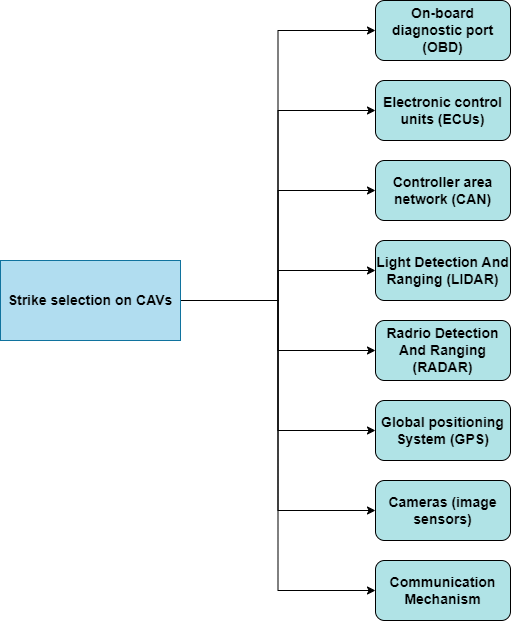
\includegraphics[scale=0.60]
  {img/Attack targets}
  \caption{The possible targets of an attack on a CAV.}   
  \label{fig:The possible targets of an attack on a CAV}
\end{figure}


\subsection{Communication Types and Protocols}
\hspace{5mm} The Internet of Things (IoT) is a technology that is still evolving and has many applications. One example of these applications is the development of intelligent infrastructure for vehicles that utilize internet-connected devices. In connection with the IoT, there is a branch of IoT called Internet of Vehicles (IoV) \cite{article23}.

\hspace{5mm} As a network of devices that communicate and share information, the IoT platform is defined as a collection of connected devices to form a network. With the development of new and improved devices and services, IoT has become a leading technology. In light of this expansion, the IoT platform has become increasingly popular and applicable to a wide variety of research fields, leading to new areas of application. VANETs, which connect vehicles to other vehicles and infrastructure, are one example of vehicular ad hoc networks. VANETs have evolved into IoVs and are expected to become the IoAVs in the near future \cite{article23}.

\hspace{5mm} VANETs, allow mobile devices/vehicles to spontaneously create networks \cite{article24}. In addition to V2V, VANETs can also be used for V2I communications \cite{article24}. As a result of such technology, road safety is enhanced; for instance, vehicles are able to communicate with each other and the network to exchange essential information during hazardous conditions. 

\hspace{5mm} In VANET technology, the following components are present: In every vehicle, there is a GPS tracking device (called OBU) to communicate with one another and with an RSU \cite{article24}. The main objective of this system is to establish wireless communications between different RSUs and OBUs. With IoV, data can be collected utilizing sensors found in vehicles or roadside units, including GPS, proximity radar, accelerometers, LiDARs, image sensors, and various performance and control modules contained in the OBU \cite{article23}.

\hspace{5mm} It is possible to collect vehicle-related data such as the vehicle's speed, its location, and its direction of movement, and roadside data such as traffic flow statistics. The collected data is then used to improve traffic management, enhance road safety, and respond more effectively to accidents.

\hspace{5mm} IVC systems and sensors are the main components of vehicular networks \cite{article23}. Vehicle networks follow the same layered architecture as other networks. Although it has a layered structure, it differs from conventional networks.

\hspace{5mm} The IoAV architecture has been proposed in several different ways. In general, the sensing layers (combining physical and data links) are classified into three groups: the network layer, the sensing layer, and the application layer \cite{article23}. A summary of the sensing layers classification can be found in Figure \ref{fig:sensing layers classification}.


\begin{figure}[H]
  \centering
  \includegraphics*[width=0.8\columnwidth]
  {img/Layer-based classification of current standards}
  \caption{sensing layers classification.}   
  \label{fig:sensing layers classification}
\end{figure}

\hspace{5mm} A three-layered architecture starts with a sensing layer at the bottom. As part of this architecture, the sensing layer is composed of the physical layer and the data link layer \cite{article23}. Information about the environment is collected by this layer through the use of available sensors \cite{article23}. In addition to driving patterns and environmental conditions, data can be collected on vehicle situations, vehicle conditions, and more.

\hspace{5mm} Regarding Network Layer, upon receiving data from the bottom layer, the application layer processes it and transmits it. Many types of network technologies are used to process the abundance of data, including LANs, wireless/wired networks, and transmission mediums such as WLANs, Bluetooth, and Zigbees \cite{article23}. Since it is responsible for providing connectivity, this layer is appropriately called the communication layer \cite{article23}. It handles V2V, V2I, pedestrian-to-pedestrian, and sensor-to-sensor communication \cite{article23}.

\hspace{5mm} As the application layer provides storage and processing for the data, it is the powerhouse of the resource. A major responsibility of the role is the management of data, storage, processing, and even the decision-making process \cite{article23}. Additionally, the layer supports big data analysis, wireless sensor networks, cloud computing, etc. The application layer and the business layer can be subdivided further within this layer. The IoAV platform is accessed through this layer. Different applications are managed through this layer, which facilitates their management.

\hspace{5mm} Roadside units, also known as RSUs, are fixed at specific locations such as roadside areas, parking lots, and intersections \cite{article24}. By connecting AVs to infrastructure and assisting in vehicle localization, its main purpose is to provide connectivity between AVs and infrastructure. Moreover, it can be used to connect vehicles to different types of RSUs.

\hspace{5mm} An established TA manages the VANET registration and communication process to ensure only valid RSUs and OBUs can register \cite{article24}. As well as providing security, it authenticates the vehicle and verifies the OBU ID.

\hspace{5mm} V2V communication, V2I communication, and V2X communication can be accomplished utilizing VANETs \cite{article24}, the details have been illustrated in Figure \ref{fig:The vehicle communication system}. V2V communication, also known as IVC, enables vehicles to communicate with one another and exchange traffic congestion, accident, and speeding information \cite{article24}. MIVC is used for long-range communication like traffic monitoring, while SIVC is used for short-range applications like lane merging and ACC. There are several advantages that come from V2V communication, including BSD, FCWS, AEB, and LDWS. The nodes (vehicles) in a V2V communication network are connected using a mesh (partial or full) topology. A SIVC or MIVC system is categorized based on how many hops are used for IVC.

\hspace{5mm} Through Vehicle-to-Infrastructure (V2I) Communication and Roadside-to-Vehicle Communication (RVC), vehicles are able to engage with Roadside Units (RSUs). \cite{article24}. This device is capable of identifying traffic signals, cameras, lane indicators, and parking meters. In an ad hoc network, the ad hoc and bidirectional communication between vehicles and the infrastructure is wireless and ad hoc. Data gathered from infrastructure enables oversight and control of traffic. These data are utilized to adjust various speed parameters, aiming to optimize fuel efficiency and regulate traffic movement. RVC systems are classified as SRVCs and URVCs depending on the infrastructure \cite{article24}. Communication services are provided only by SRVC systems at hotspots, such as gas stations and parking spaces, while URVC systems provide coverage throughout the road even at high speeds. Due to this, URVC requires significant investment in order to maintain network coverage.

\hspace{5mm} With the V2X concept, vehicles can communicate omnidirectionally with other vehicles (V2V), with infrastructure (V2I), with pedestrians (V2P), and with networks (V2N/V2C) that connect to networks and clouds \cite{article25}. Using this technology, pedestrians, vehicles, road networks, and cloud environments can be connected. Not only can V2X assist vehicles in obtaining information and promote innovation and application of automated driving technology, but it can also contribute to the creation of an intelligent transport network, and it can encourage the development of new modes and new forms of automobiles and transportation services in the future \cite{article25}. Traffic efficiency, pollution reduction, resource conservation, accident prevention, and traffic management can all be improved with this technology.

\hspace{5mm} LTE-V2X and DSRC are the two main types of communications technology used for V2X at present \cite{article25}. There are several standards that make up the DSRC system, including IEEE and SAE guidelines. DSRC uses the 802.11p protocol at both the physical and medium access control layers \cite{article25}. This protocol enables vehicles to broadcast relevant security information directly to neighboring vehicles and pedestrians by simplifying authentication, associated processes, and data transmission before transmitting data.


\begin{figure}[H]
  \centering
  \includegraphics*[width=0.8\columnwidth]{img/VC}
  \caption{The vehicle communication system (VC).}   
  \label{fig:The vehicle communication system}
\end{figure}


\hspace{5mm} Through different wireless technologies, an AV can communicate with other vehicles and network infrastructure. When the AV is engaged in V2X communication, real-time data (audio/video) may be transmitted and received in real-time; in case of fog or an accident, warning information can be exchanged with neighboring vehicles in real-time. Using Figure \ref{fig:VANET technologies}, we illustrate how autonomous vehicle wireless technologies can be differentiated by their transmission ranges.

\begin{figure}[H]
  \centering
  \includegraphics*[width=1.1\columnwidth]{img/VANET technologies}
  \caption{A variety of VANET technologies are being considered for AVs.}   
  \label{fig:VANET technologies}
\end{figure}


\hspace{5mm} Bluetooth Technology is a notable example of Short-Range Communication Technology \cite{article24}. Vehicular networks can utilize wireless short-distance communication technologies like Bluetooth, which is based on the IEEE 802.15.1 standard. Operating in the 2.4 GHz frequency band, this wireless network can provide data transmission speeds of up to 14Mbps over diverse distances. As Bluetooth propagates, it varies in range as a result of antenna sensitivity, gain, and propagation conditions.\par

\hspace{5mm} IoT networks are needed to be low-cost and low-power, so ZigBee technology was developed \cite{article24}. Approximately 250 kbps of data can be transferred over a distance of 100 m with the supported connectivity range \cite{article24}. In addition to being known as IEEE 802.15.4, it is also referred to as LRWPAN and is operated at different frequencies (868 MHz, 902–968 MHz, and 2.4 GHz) \cite{article24}.\par

\hspace{5mm} It is noteworthy that DSRC technologies are part of medium-range communication technologies \cite{article24}. An example of this is DSRC, which is referred to as WAVE. It uses WAVEs to provide reliable communication between vehicles and vehicle infrastructures. In order to create a wide area network between vehicles, the technology can be deployed in OBUs and RSUs \cite{article24}. Vehicles communicate using DSRC when communicating with one another through V2V communication. As well as V2I communication, it can be used to send traffic signals as well as accident alerts to vehicles over the network infrastructure.

\hspace{5mm} As far as Long Range Communications Technology is concerned, C-V2X Technology stands out \cite{article24}. Cellular networks are used to connect vehicles with their surroundings. Release 14 of 3GPP introduced C-V2X technology, and release 15 developed it further in order to meet 5G communication criteria \cite{article24}.
As a result, C-V2X is extremely reliable, capable of communicating between vehicles at high speeds, is capable of operating perfectly in dense traffic conditions, In doing so, it mitigates the congestion problems related to DSRC, and facilitates both close and extended distance communication between vehicles and the Roadside Unit (RSU).

\hspace{5mm} Lastly, with 5G-NR, developed by 3GPP, data rates increase, latency decreases, and devices can communicate more effectively \cite{article24}.



\subsection{Mapping and Localization}

\hspace{5mm} The field of mapping is extremely important in the field of Intelligent Transportation Systems (ITS) and has increasingly been studied. An example of one of the most widely used mapping techniques is road network mapping, which is based on the network of roads in a given area. There are numerous applications of it, including vehicle localization, route planning, and navigation control. The road network is typically extracted from Google Maps or OSM, unlike OGM, which is constructed through the use of range measurements like LiDARs or SONARs \cite{article31}.

\hspace{5mm} With the ability to build a map, we now have access to various other applications, including vehicle localization. GPS is primarily used in ITS applications such as vehicle positioning, which is a highly crucial task. The data is, however, affected by a wide range of error sources, which makes it difficult to calculate accurate trajectory data. The data must be linked to the road network through Map Matching in order to be useful for vehicle localization. Based on noisy GPS measurements, map matching determines the actual route the vehicle took to arrive at its destination \cite{article31}. Many methods are used to implement map matching, but the HMM and an algorithm based on it are the most widely used \cite{article31}. Based on knowledge of the road networks' connectivity, the HMM can provide reasonable routes based on a probability-based approach \cite{article31}. Generally, the route planner is already aware of the route that the vehicle should follow in autonomous driving applications. As a result, complex HMMs are considered unsuitable for such applications.

\hspace{5mm} There are three types of localization on highways: Road-level localization (RLL), Ego-lane level localization (ELL), and Lane-level localization (LLL) \cite{article32}.

\hspace{5mm} In order to perform the RLL, digital maps are used (e.g., Google, OSM, and Waze) \cite{article32}. Geodetic coordinates (latitude, longitude, and altitude) are retrieved using GNSS receivers \cite{article32}. A Map-Matching procedure is then performed to determine the right road, matching the location of the ego-vehicle. While localization is obtained with meters of accuracy, there is still a lot of uncertainty.

\hspace{5mm} When it comes to \textit R\textit L\textit L, almost all vehicles are equipped with positioning devices that allow drivers to know where their vehicles are in the world. These positioning devices are inherently inaccurate, which makes this estimation very noisy. A correcting process is required to resolve this problem, which matches the vehicle position with a map-based road network. A map-matching technique is used to achieve this \cite{article32}.

\hspace{5mm} In addition to identifying the vehicle's physical location, map-matching improves its position accuracy when spatial road network data is available. As a result, the Map-Matching algorithm is the one that determines the RLL knowledge. Numerous applications require RLLs as prerequisites \cite{article32}.


\hspace{5mm} Online Map-Matching has been a major subject of research since GPS became available in the 1990s because of its importance to the RLL \cite{article32}. In terms of map-matching techniques, there are two main categories: online and offline \cite{article32}. When Map-Matching is performed online, it occurs in a streaming mode. As a result, real-time applications require an adequate procedure. To achieve full Map-Matching in offline Map-Matching, the trajectory must be completed before Map-Matching is performed.

\hspace{5mm} There are four categories of map-matching techniques from a methodological standpoint, namely geometric, topological, probabilistic, and advanced \cite{article32}. The map-matching methods have, however, been outperformed and new technologies have emerged over the last several years, resulting in the classification becoming obsolete. The existing Map-Matching methods are classified into two categories: Probabilistic Models and Deterministic Models \cite{article32}. The categories are further divided into subcategories \cite{article32}. Figure \ref{fig:Map-Matching} depicts each category in detail.


\begin{figure}[H]
  \centering
  \includegraphics*[width=1.1\columnwidth]{img/Map-Matching}
  \caption{Classification using map-matching techniques can be divided into two main categories - deterministic and probabilistic.}   
  \label{fig:Map-Matching}
\end{figure}


\hspace{5mm} With regard to \textit E\textit L\textit L, a vehicle's awareness of the road on which it is traveling is not sufficient for some applications, such as lane-keeping. \cite{article32}. It is essential that these systems know where the host lane in the road is so that they can provide appropriate maneuvering instructions and maintain vehicle safety. More accurate localization of AVs is also needed, which is possible by analyzing the longitudinal and lateral positions of the vehicle in the ego lane \cite{article32}. Overtaking maneuvers, for example, require flawless knowledge of the vehicle's lateral position with respect to the ego-lane marking in order to detect if it should overtake the obstacle.


\hspace{5mm} The majority of researchers use lane marking detection to determine the location of ego lanes at the level of an individual \cite{article32}. A modular pipeline approach, a model-driven approach, or a monolithic end-to-end approach can all be classified as existing approaches to lane marking detection \cite{article32}. A model-driven approach is the standard for lane marking detection. In general, lane marking detection should be broken down into independent modules that can be tested independently. In modular pipelines, intermediate representations are comprised of human-interpretable elements that are helpful in understanding how a system fails \cite{article32}. It has been observed that modular methods inherently lack suitability for tasks such as identifying lanes based on intermediate representations built by humans \cite{article32}. Models based on ANNs that learn from start to finish are an alternative to modular pipelines.

\hspace{5mm} Regarding the \textit L\textit L\textit L, for an autonomous vehicle to function properly, it must be able to evaluate the road environment in which it operates. In order to evaluate the situation properly, it is crucial to comprehend some essential components of localization levels. The concept of LLL  is a broad term that refers to two distinct topics\cite{article32}. As a first step, the ego lane should be determined, i.e., the lane that the vehicle is currently traveling on. Furthermore, it may refer to determining the vehicle's lateral position inside the overall road. In addition to LLL, there are various systems that can help AVs obtain it. GNSS receivers can be used by some systems to locate the ego-vehicle on the road \cite{article32}. With the IMU, proprioceptive sensors can compensate for the lack of accuracy provided by classical GNSS, which can be caused by poor satellite signals, high precision dilution, or multi-path in urban scenes \cite{article32}.



\newpage

\section{Results}
\label{results}
\hspace{5mm} This section presents the results of the review of the selected articles and comprises different sections that aim to answer the proposed research questions. The first part pertains to types of methods and techniques, providing information to answer the first research question. The second part presents evidence to demonstrate the results, aiming to answer the second research question. Finally, we discuss the limitations identified in the proposed methods to answer the last research question. As this review considers only studies published from 2019 to 2022, the selected studies span this period. Table ~\ref{tab:primary_studies} illustrates the distribution of these studies over this time span. Moreover, the references of all the selected documents are presented in Table \ref{tab:Full Reference}.


\begin{table}[hbt!]
\caption{Selected primary studies}
\label{tab:primary_studies}
\resizebox{\textwidth}{!}{%
\begin{tabular}{|l|l|l|l|}
\hline
\rowcolor[HTML]{00D2CB} 
\multicolumn{1}{|c|}{\cellcolor[HTML]{00D2CB}{\color[HTML]{000000} \textbf{Id}}} & \multicolumn{1}{c|}{\cellcolor[HTML]{00D2CB}{\color[HTML]{000000} \textbf{Title}}}                                        & \multicolumn{1}{c|}{\cellcolor[HTML]{00D2CB}{\color[HTML]{000000} \textbf{year}}} & \multicolumn{1}{c|}{\cellcolor[HTML]{00D2CB}{\color[HTML]{000000} \textbf{Type}}} \\ \hline
S1                                                                               & Adaptive Driving Assistant Model (ADAM) for Advising Drivers of Autonomous Vehicles                                       & 2022                                                                              & Article                                                                           \\ \hline
S2                                                                               & MADRaS : Multi-Agent Driving Simulator                                                                                    & 2021                                                                              & Article                                                                           \\ \hline
S3                                                                               & Crossroads+: A Time-aware Approach for Intersection Management of Connected Autonomous Vehicles                           & 2020                                                                              & Article                                                                           \\ \hline
S4                                                                               & Cooperative Intersection Crossing Over 5G                                                                                 & 2021                                                                              & Article                                                                           \\ \hline
S5                                                                               & Semi-Direct Monocular Visual-Inertial Odometry Using Point and Line Features for IoV                                      & 2022                                                                              & Article                                                                           \\ \hline
S6                                                                               & Design and Analysis of Delay-Tolerant Intelligent Intersection Management                                                 & 2020                                                                              & Article                                                                           \\ \hline
S7                                                                               & Autonomous Vehicle: Security by Design                                                                                    & 2021                                                                              & Article                                                                           \\ \hline
S8                                                                               & Collaborative Analysis Framework of Safety and Security for Autonomous Vehicles.                                          & 2019                                                                              & Article                                                                           \\ \hline
S9                                                                               & Trajectory Planning and Safety Assessment of Autonomous Vehicles Based on Motion Prediction and Model Predictive Control  & 2019                                                                              & Article                                                                           \\ \hline
S10                                                                              & RFAP: A Revocable Fine-Grained Access Control Mechanism for Autonomous Vehicle Platoon                                    & 2022                                                                              & Article                                                                           \\ \hline
S11                                                                              & A Methodology for the Design of SafetyCompliant and Secure Communication of Autonomous Vehicles                           & 2019                                                                              & Article                                                                           \\ \hline
S12                                                                              & LiDAR Data Integrity Verification for Autonomous Vehicle                                                                  & 2019                                                                              & Article                                                                           \\ \hline
S13                                                                              & RACE: Reinforced Cooperative Autonomous Vehicle Collision Avoidance                                                       & 2020                                                                              & Article                                                                           \\ \hline
S14                                                                              & Photonic-Radar Based Multiple-Target Tracking under Complex Traffic-Environments                                          & 2020                                                                              & Article                                                                           \\ \hline
S15                                                                              & Achieving Lightweight and Privacy-Preserving Object Detection for Connected Autonomous Vehicles                           & 2022                                                                              & Article                                                                           \\ \hline
S16                                                                              & Semantic Point Cloud-Based Adaptive Multiple Object Detection and Tracking for Autonomous Vehicles                        & 2021                                                                              & Article                                                                           \\ \hline
S17                                                                              & An enhanced conceptual security model for autonomous vehicles                                                             & 2020                                                                              & Article                                                                           \\ \hline
S18                                                                              & Virtual Traffic Light Implementation on a Roadside Unit over 802.11p Wireless Access in Vehicular Environments            & 2022                                                                              & Article                                                                           \\ \hline
S19                                                                              & Edge Computing for Autonomous Driving: Opportunities and Challenges                                                       & 2019                                                                              & Article                                                                           \\ \hline
S20                                                                              & Unified Biometric Privacy Preserving Three-Factor Authentication and Key Agreement for Cloud-Assisted Autonomous Vehicles & 2020                                                                              & Article                                                                           \\ \hline
S21                                                                              & Safe and Effective Transfer of Feedback Control Signals Based on Vision                                                & 2021                                                                              & Article                                                                           \\ \hline
S22                                                                              & Chaos-based privacy preserving vehicle safety protocol for 5G Connected Autonomous Vehicle networks                       & 2020                                                                              & Article                                                                           \\ \hline
S23                                                                              & Developing an Evaluation Method for Potential Cyber Threat Severity to Connected and Autonomous Vehicles                     & 2020                                                                              & Article                                                                           \\ \hline
S24                                                                              & Cybersecurity challenges in vehicular communications                                                                      & 2019                                                                              & Article                                                                           \\ \hline
\end{tabular}%
}
\end{table}




\newpage
\subsection{Types of Methods and Techniques (RQ1) }
\hspace{5mm} This section presents the types of methods and techniques used in selected primary studies. The information provided in Table~\ref{tab:Proposed_Technique} displays different types of methods/techniques primarily used or developed in the selected studies. Because the table doesn't present comprehensive information, the remainder of this subsection provides an in-depth description of the studies.


\begin{table}[hbt!]
\caption{Proposed Techniques}
\label{tab:Proposed_Technique}
\resizebox{\textwidth}{!}{%
\begin{tabular}{|l|l|}
\hline
\rowcolor[HTML]{00D2CB} 
\multicolumn{1}{|c|}{\cellcolor[HTML]{00D2CB}{\color[HTML]{000000} \textbf{ID}}} & \multicolumn{1}{c|}{\cellcolor[HTML]{00D2CB}{\color[HTML]{000000} \textbf{Technique}}}   \\ \hline
S1                                                                               & Adaptive Driving Assistant Model (ADAM)                                                  \\ \hline
S2                                                                               & MADRaS: Multi-Agent Driving Simulator                                                   \\ \hline
S3                                                                               & Crossroads+                                                                              \\ \hline
S4                                                                               & Control algorithm and a communication paradigm over 5G networks                          \\ \hline
S5                                                                               & Semi-Direct Monocular Visual-Inertial Odometry using Point and Line Features (SDMPL-VIO) \\ \hline
S6                                                                               & Delay-tolerant protocol for general multi-lane intersection management                                          \\ \hline
S7                                                                               & Security-by-design framework for AV                                                      \\ \hline
S8                                                                               & Collaborative Analysis Framework                                                         \\ \hline
S9                                                                               & Trajectory Planning and Safety Assessment                                                \\ \hline
S10                                                                              & RFAP: A Revocable Fine-Grained Access Control                                            \\ \hline
S11                                                                              & Adopted the Arrowhead Framework and a contract-based approach                            \\ \hline
S12                                                                              & Semi-fragile data hiding-based technique                                                 \\ \hline
S13                                                                              & RACE: Reinforced Cooperative Autonomous Vehicle Collision Avoidance                      \\ \hline
S14                                                                              & Photonic-Radar Based Multiple-Target Tracking                                            \\ \hline
S15                                                                              & Privacy-preserving object detection (P2OD) framework                                     \\ \hline
S16                                                                              & A semantic point cloud-based adaptive MODT system                                        \\ \hline
S17                                                                              & Conceptual model of autonomous vehicles                                                  \\ \hline
S18                                                                              & Road-Side Unit-based Virtual Intersection Management (RSU-VIM)                           \\ \hline
S19                                                                              & Review edge computing system
designs, V2X applications, and autonomous vehicle security.                                             \\ \hline
S20                                                                              & Cloud-centric Three-factor Authentication and Key Agreement protocol (CT-AKA)            \\ \hline
S21                                                                              & Pipeline of cryptographic operations                                                     \\ \hline
S22                                                                              & 5G radio network architecture                                                            \\ \hline
S23                                                                              & Identified cyber attacks on CAV                                                          \\ \hline
S24                                                                              & Three-layer framework (sensing, communication and control)                               \\ \hline
\end{tabular}%
}
\end{table}




\begin{figure}[H]
  \centering
  \includegraphics*[width=1.1\columnwidth]{img/Types of Methods and Techniques overview}
  \caption{Types of Methods and Techniques overview.}   
  \label{fig:Types of Methods and Techniques overview}
\end{figure}

\hspace{5mm} Figure ~\ref{fig:Types of Methods and Techniques overview} offers an overview of the types of methods and techniques developed and utilized in the selected articles, depicted in percentages. It is worth mentioning that more than 50\% of the studies develop methods in the field of security and object detection and localization techniques for AVs. This finding suggests that these two fields are trending in recent years. \par

\subsubsection{Advanced Data Processing and Decision-Making Algorithms}
\hspace{5mm} Numerous studies propose advanced data processing techniques and decision-making algorithms to enhance autonomous vehicle functionality and safety. For instance, one study (S1) proposes an architecture for adaptive autonomous driving assistance, employing a two-layer fusion model and a two-stage development process involving predictive trust in automation and ADAMs. Machine learning techniques such as ANN, SVM, and RF are instrumental in this approach \cite{s1}. Another study (S2) presents MADRaS, an open-source motion planning simulator used for developing and evaluating autonomous driving algorithms, relying heavily on the PPO algorithm \cite{s2}. The study (S3) develops Crossroads+, a time-sensitive intersection management approach accounting for various factors, including network delays and the physical behavior of CAVs \cite{s3}.\par
The study (S9) utilizes Monte Carlo simulations to predict the probabilistic occupancy rates of an object, creating a map of probability statistics that correspond to actual scenarios. This approach accounts for the motion predictions of other traffic participants, enabling the model to handle dynamic environments with high requirements on perceptual systems effectively \cite{s9}.

\newpage
\subsubsection{Communication and Networking Paradigms}
\hspace{5mm} A few studies (S4, S18) focus on developing new communication paradigms to facilitate effective communication between AVs and infrastructures. The study (S4) presents a low-latency generalized message exchange system, Hermes, leveraging the simplicity of Client-Server and the efficiency of Multicast communication \cite{s4}. The study (S18) proposes a VIM system using RSUs through 802.11p, adapted from existing virtual traffic light methodologies \cite{s18}.\par
One study (S22) proposes a 5G radio network architecture that utilizes multiple radio access technologies in conjunction with CRAN capabilities to preserve privacy on CAV networks without compromising security. The study also proposes a reliable, secure, and privacy-preserving protocol for disseminating messages in CAV networks \cite{s22}. Edge computing and V2X applications are explored in a study (S19). The authors review state-of-the-art approaches in edge computing system designs, V2X applications, and autonomous vehicle security, discussing recent advancements and challenges in building edge computing systems for AVs \cite{s19}


\subsubsection{Security Approaches and Techniques}
\hspace{5mm} The topic of security is a major cause for concern in AVs, with multiple studies (S7, S8, S10, S11, S17, S20, S21, S23, S24) proposing various security approaches and techniques. One study (S7) derives security objectives and controls from AV safety requirements and proposes AV security approaches within a socio-technical framework. The paper focuses on the integration of security measures into the design and development of autonomous vehicles. By considering security from the early stages, adopting secure design principles, and addressing the unique security challenges, the paper aims to enhance the overall security and resilience of autonomous vehicles in the face of potential threats and attacks \cite{s7}. Another study (S8) proposes a method for integrating safety and security with international standards like ISO 26262 and SAE J3061. Due to the automation levels of DAS, TARA and HARA should correspond with each DAL, i.e., TARA and HARA must consider particular properties of each DAL \cite{s8}. Similarly, the study (S11) takes a contract-based approach to specify safety, combined with the Arrowhead Framework to support security. This contract-based approach can neatly distinguish between the responsibilities of different components in the form of assumptions and guarantees, expressed as assertions in the pattern-based BCL language \cite{s11}. A conceptual model of AVs focusing on their assets, vulnerabilities, and threats is proposed in the study (S17) \cite{s17}. Lastly, the study (S20) introduces a cloud-centric three-factor authentication and CT-AKA to ensure secure access to the cloud and AVs \cite{s20}.\par
The study (S10) proposes a Revocation-based Attribute-based Access Control mechanism (RFAP) for AVPs. This mechanism achieves fine-grained access control through encryption and facilitates immediate revocation and secure outsourced decryption through ECUs. The proposal includes four PPT algorithms: Setup, KeyGen, Encrypt, and Decrypt. Similarly, the study (S21) proposes a new stream cipher, demonstrating better performance than past block ciphers and efficient authenticated encryption, particularly useful for the safe and efficient transfer of sensor data between computing devices \cite{s10}.\par
The study (S23) identifies significant CAV cyberattacks, conducts an analysis of the target asset, possible risks, and consequences for each identified cyberattack, and suggests mitigation methods \cite{s23}. Similarly, the study (S24) proposes a three-layer framework to enhance the understanding of automotive security threats in the context of modern vehicles that can connect to an external infrastructure and increasingly use V2X communication technologies. The three layers include a sensing layer, composed of vehicle dynamics and environmental sensors vulnerable to various attacks; a communication layer, which includes both in-vehicle and V2X communications, susceptible to a range of attacks; and a control layer, which enables autonomous vehicular functionality and can be compromised by attacks targeting the lower two layers \cite{s24}.

\subsubsection{Object Detection and Localization Techniques}
\hspace{5mm} Object detection and localization are addressed in various studies (S5, S14, S15, S16). The study (S5) develops an SDMPL-VIO for precise vehicle localization \cite{s5}. Similarly, the study (S15) proposes an integrated approach to the extraction of features and bounding boxes from objects in an image using multiple secure computing protocols, while the study (S16) proposes an adaptive MODT system based on SPCs \cite{s15}. The study (S14) develops a linear frequency-modulated continuous-wave photonic radar to carry out a radar cross-section-based tracking of multiple mobile targets in complex traffic scenarios under various weather conditions such as fog, cloud, and rain \cite{s14}.

\subsubsection{Sensor Data Integrity Verification and Tampering Detection}
\hspace{5mm} Ensuring sensor data integrity and detecting tampering is the focus of two studies (S12, S13). Both propose a semi-fragile data hiding-based technique for verifying the integrity of sensor data in real time, as well as detecting and localizing tampering in real-time. They use a 3-dimensional QIM-based data hiding for inserting binary watermarks into LiDAR data \cite{s12}, \cite{s13}.

\subsubsection{Intersection and Traffic Management}
\hspace{5mm} Two studies (S3, S6) present solutions for intersection and traffic management. The study (S3) proposes Crossroads+, a time-sensitive intersection management approach taking network delays and CAVs' physical behavior into account. On the other hand, the study (S6) develops a delay-tolerant protocol for managing intersections with several lanes in each direction, aiming to minimize deadlocks and increase efficiency \cite{s3}, \cite{s6}.

\newpage

\subsection{Evidence to Demonstrate the Result (RQ2)}
\hspace{5mm} This section presents the evidence and evaluation methods that the studies used to demonstrate and evaluate their results. Moreover, it can be mentioned that as the studies utilize different limitation techniques, we will explain them based on the categorization.


\begin{figure}[H]
  \centering
  \includegraphics*[width=1.1\columnwidth]{img/Overview of evidence for demonstrating the result}
  \caption{Overview of evidence for demonstrating the result.}   \label{fig:Overview of evidence for demonstrating the result}
\end{figure}

Figure ~\ref{fig:Overview of evidence for demonstrating the result} provides an overview of the different evaluation methods in the selected articles in percentage. We mention that simulation-based evaluations and experimental real-world testing are more utilized in the process of evaluating the results.


\subsubsection{Simulation-Based Evaluation}
\hspace{5mm} Several studies utilize various simulation tools to evaluate their proposed models, techniques, or frameworks. One study (S2) uses MADRaS, an open-source MADRaS, to evaluate autonomous driving motion planning algorithms. Experiments simulate complex driving scenarios and various control modes \cite{s2}. Similarly, another study (S3) uses a two-pronged approach, employing real-world experiments and a custom-built simulator to validate their Crossroads+ technique for managing intersections \cite{s3}. The researchers in the study (S6) extend the SUMO traffic simulation suite to analyze the performance of their delay-tolerant intersection management protocol \cite{s9}. Simulation-based quantitative analysis is also used in the study (S9), where Monte Carlo simulation is employed for predicting the probabilistic occupancy of other traffic participants \cite{s9}.\par
The research team in the study (S10) uses the Veins traffic simulator with the PLEXE package to evaluate the efficiency and resistance of their RFAP mechanism to continuous jamming attacks \cite{s10}. Finally, the last study (S13) uses TORCS to evaluate their proposed RACE framework, focusing on metrics such as collisions, scalability, and latency. In the study (S14), a wide range of traffic scenarios is modeled using MATLAB™ software to simulate different types of mobile targets with varying radar cross-sections, testing the radar’s performance in both normal and complex traffic scenarios \cite{s13}. Similarly, the study (S15) utilizes a PyCharm simulation platform to execute secure computing protocols within the P2OD framework. The study (S16) incorporates the Carla simulator, providing a semantic point cloud labeled as ground truth, to complement the KITTI data set in evaluating their tracking performance \cite{s15}. Lastly, the study (S24) evaluates the security of vehicular communications and proposes the use of machine learning and blockchain technologies through various simulation platforms \cite{s24}.\par
The researchers in the study (S7) use software simulations to evaluate the security of AVs under three key attack scenarios \cite{s7}. Similarly, the study (S10) combines theoretical and experimental analyses to demonstrate the results of their AVP security solution, RFAP \cite{s10}. The researchers in the study (S11) employ a contract-based approach for specifying safety, incorporating it into the design flow with the Arrowhead Framework to support security \cite{s11}.

\subsubsection{Experimental Real-World Testing}
\hspace{5mm} Some studies employ real-world testing or demonstration to evaluate their proposed techniques. In the study (S1), telemetry data from automated vehicles are used in combination with machine learning techniques to develop a model predicting drivers’ trust in automation \cite{s1}. The study (S4) tests a control algorithm and communication paradigm over 5G networks at the AstaZero proving ground in Goteborg, Sweden \cite{s4}. The study (S7) conducts physical testing to evaluate the security of AVs under three key attack scenarios \cite{s7}. The physical demonstration is also used in one of the studies (S11), where model cars are used to showcase a platooning autonomous vehicle system \cite{s11}. In the study (S17), a multi-layered approach is applied to evaluate the vulnerabilities of AVs to cyber-attacks, focusing on a specific instance of a cyber-attack on a Jeep Cherokee to understand potential attack surfaces \cite{s17}. Similarly, the study (S23) examines the severity of potential cyber-attacks on CAVs and proposes mitigation methods \cite{s23}.

\subsubsection{Data Analysis and Machine Learning Techniques}
\hspace{5mm} Several studies utilize data analysis or machine learning techniques to evaluate their proposals. The study (S1) uses machine learning models to predict trust in automation based on various vehicle attributes \cite{s1}. The mentioned models are two layers of sensor fusion models. The first layer includes models for speed conditions, road conditions, driver distraction, and trust prediction. The second layer integrates the outputs from the first stage to trigger appropriate voice instructions, enhancing driver safety \cite{s1}. The researchers in the study (S5) employ an SDMPL-VIO model for vehicle localization, tested on both indoor (EuRoC) and outdoor (KITTI) datasets \cite{s5}. In the study (S8), the researchers use an integrated safety and security method (S12) based on international vehicle safety and security standards for analyzing potential failures and attacks on LiDAR \cite{s8}, \cite{s12}. The use of mathematical proofs is also evident in the study (S6), where the researchers formally prove the safety, liveness, and deadlock-free properties of their protocol \cite{s6}.

\subsubsection{Use of Data-sets}
\hspace{5mm} Data sets are utilized as a primary method of evaluation in multiple studies (S15, S16). The researchers in the first study (S15) use the KITTI data set to train and test the P2OD framework. Evaluating the computational cost, communication overhead, and accuracy of various detection and classification phases \cite{s15}. Similarly, the study (S16) employs the KITTI data set in conjunction with a simulator to verify tracking performance in real-world scenarios \cite{s16}. In the study (S12), A technique based on semi-delicate data hiding is utilized for the real-time validation of sensor data integrity and for identifying and locating any tampering. The method is evaluated on a benchmarking LiDAR dataset \cite{s12}.

\subsubsection{Comprehensive Review}
\hspace{5mm} In the study (S19), The researchers utilize a comprehensive review and analysis of existing technologies and methodologies in their evaluation. They conduct an extensive study of advancements in edge computing system designs, V2X applications, and autonomous vehicle security \cite{s19}.

\subsubsection{Histograms and Key Space Analysis}
\hspace{5mm} The study (S22) uses histograms and key space analysis to verify the security of the proposed encryption algorithm, measuring its computational time cost and impact on network latency \cite{s22}.

\subsubsection{Prototyping and Hardware-Based Evaluation}
\hspace{5mm} In the study (S18), the researchers evaluate their RSU-VIM system using a prototype setup that includes hardware such as SDRs, an FPGA, and a Raspberry Pi. The system's performance is evaluated based on metrics such as system delay, packet transmission delay, and reliability \cite{s18}.

\subsubsection{Computational Analysis and Protocol Verification}
\hspace{5mm} In two different studies (S20, S21), computational analysis and protocol verification serve as evaluation methods. The first study (S20) employs Proverif v1.97, an automatic cryptographic protocol verifier, to assess the security of the proposed CT-AKA protocol. The protocol’s efficiency is analyzed from two aspects - computational time and communication cost \cite{s20}. In the study (S21), a series of experiments is run on embedded computers to compare the performance of different cryptographic methods, with latencies calculated for various schemes \cite{s21}.

\newpage

\subsection{Limitations (RQ3)}
\hspace{5mm} This section presents the limitations and open problems of existing methods that could potentially point to interesting future research directions for practitioners and researchers in the context of improving the safety and security of AVs. Moreover, it can be mentioned that as the studies face different limitations, we explain based on the categorization.

\begin{figure}[H]
  \centering
  \includegraphics*[width=1.1\columnwidth]{img/Overview of limitations result}
  \caption{Overview of limitations result.}   \label{fig:Overview of limitations result}
\end{figure}

Figure ~\ref{fig:Overview of limitations result} provides an overview of the different limitations identified in the selected articles in percentage. It is evident that there are two significant problems that researchers face 1) simulation and testing and 2) security concerns and cyber attacks. \par

\begin{table}[H]
\centering
\caption{Mapping of Limitations in Selected Studies}
\label{tab:limitation_mapping}
\begin{tabularx}{\textwidth}{|X|c|c|}
\hline
\rowcolor[HTML]{00D2CB} 
\textbf{Limitations} & \textbf{Studies} & \textbf{Total} \\
\hline
Scarcity of Data-sets & S1,S4,S5,S16,S18 &  5 \\
\hline
Communication Challenges & S3,S4,S6,S10,S13 & 5    \\
\hline
Hardware and Software Limitations & S5,S7,S10,S12,S15,S16 & 6   \\
\hline
Performance and Real-Time Applications & S16,S18 & 2  \\
\hline
Assumptions and Simplifications & S3,S6,S7,S9,S10,S11,S13 & 7   \\
\hline
System Design and Implementation & S19,S21,S2 & 3    \\
\hline
Generalizability and Future Research & S1,S19,S23,S24 & 4   \\
\hline
Simulation and Testing & S2,S3,S6,S9,S10,S12,S13,S14,S16 & 9    \\
\hline
Security Concerns and Cyber Attacks & S8,S10,S11,S17,S19,S20,S23,S24 & 8    \\
\hline
Scalability and Traffic Conditions & S15,S22 & 2   \\
\hline
\end{tabularx}
\end{table}

\hspace{5mm} Table~\ref{tab:limitation_mapping} presents the reference mapping of the categories of limitations identified in the articles. Given that some articles encounter multiple limitations, they appear in different categories concurrently and are examined separately according to their limitation types.

\subsubsection{Scarcity of Data-sets}
\hspace{5mm} By analyzing the results of the SLR, we find that existing studies face the limitation of the insufficient data set or diversity of data set to evaluate their proposed method. This limited diversity and quantity hinder the ability to train and test autonomous systems on various real-world scenarios, potentially leading to performance gaps when facing unfamiliar or rare situations.\par
Three of the studies (S1, S4, S5) have limitations because either there is insufficient data or data has to be generated to make up for the lack of it. This scarcity affects the evaluation of models and possibly the generalizability of the findings. While 2 of the studies (S1, S5) use generated data and still find satisfactory results, the authors acknowledge the need for more subject data to improve model accuracy \cite{s1}, \cite{s5}. Another study's (S4) experimental setup is limited to a controlled environment and a few vehicles. Hence the results might not fully reflect real-world conditions \cite{s4}.\par
The two studies (S16 and S18) discuss limitations related to the data sets used in the studies. In one of the studies (S16), the limitation arises because the KITTI tracking data set does not contain areas visible to the camera in front of the ego vehicle, and in another study (S18), the researchers use randomly generated traffic data rather than real-world intersection data, which may not fully represent real-world scenarios \cite{s16}, \cite{s18}.


\subsubsection{Communication Challenges}
\hspace{5mm} By inspecting the selected articles, we identify some limitations related to communication challenges. 5 out of 24 studies (S3,S4,S6,S10,S13) mention limitations related to communication technology. The challenges they face include the RTD causing discrepancies in communication (S3), degradation of communication performance due to urban structures (S4), assumptions about communication delays (S6), security concerns with the ECUs (S10), and assumptions about the robustness of VANETs (S13) \cite{s3}, \cite{s4}, \cite{s6}, \cite{s10}, \cite{s13}.

\subsubsection{Hardware and Software Limitations}
\hspace{5mm} Several studies (S5, S7, S10, S12, S15, S16) mention limitations related to the hardware and software used. This ranges from time-consuming feature extraction and accumulation of errors (S5), specific system configurations that may not reflect different hardware setups (S7), reliance on specific DL models (S12), computational costs, and high communication overheads (S15), to the performance of the PCSS network affecting the overall tracking performance (S16) \cite{s5}, \cite{s7}, \cite{s10}, \cite{s12}, \cite{s15}, \cite{s16}.

\subsubsection{Performance and Real-Time Applications}
\hspace{5mm} Based on the analysis of SLR-selected studies, two studies (S16, S18) highlight limitations regarding real-time application and system performance. The first study (S16) mentions that the performance of their PCSS network can affect the tracking performance of the system. It also states that the system speed drops to about seven FPS with RangeNet++, which might be a challenge for real-time applications \cite{s16}. Similarly, the second study (S18) mentions an increase in delay due to the GNU radio software, which could affect the real-time functionality of the system \cite{s18}.

\subsubsection{Assumptions and Simplifications}
\hspace{5mm} By checking the result of selected studies, we note limitations due to assumptions or simplifications made in several studies (S3, S6, S7, S9, S10, S11, S13). These include assumptions about vehicles strictly adhering to instructions (S3), modeling of communication delays (S6), assuming a semi-trusted and easy-to-compromise edge computing unit (S10) \cite{s3}, \cite{s6}, \cite{s10}. The other found assumptions are about vehicle authentication processes (S11), disregarding the specifics of the communication technology used (S13), and assuming constant longitudinal velocity during lane-change maneuvers (S9) \cite{s11}, \cite{s13}, \cite{s9}.

\subsubsection{System Design and Implementation}
\hspace{5mm} System Design and Implementation emerges as one of the identified limitations that researchers face during their research. Three articles (S19, S21, S24) highlight limitations in the design and implementation of their systems. The first study (S19) highlights the need for further research to improve the edge computer architecture for autonomous driving and the design of run-time layers for efficient workload mapping \cite{s19}. The second study (S21) faces limitations with the use of compression and decompression, which offset the potential gains by reducing the data size \cite{s21}. Lastly, the third study (S24) points out that some properties of the blockchain are too resource-intensive for onboard hardware to handle, limiting its implementation to more powerful MECUs instead of ECUs \cite{s24}.

\subsubsection{Generalizability and Future Research}
\hspace{5mm} Different studies (S17, S19, S23, S24) mention limitations regarding the generalizability of their findings and the need for future research. The findings of the study (S17) are based on a single case study, which may not be applicable to other autonomous vehicles with different designs or security protocols \cite{s17}. The study (S19) underscores the need for more research in defining attack surfaces against autonomous driving edge computing ecosystems \cite{s19}. The study (S23) discusses potential cyber-attacks only in the context of existing CAV technologies and traditional cyber attacks \cite{s23}. The study (S24) identifies the need to optimize the architecture of these models due to the hard limits on computing, memory, and power usage of automotive platforms \cite{s24}.

\subsubsection{Simulation and Testing}
\hspace{5mm} Simulations play a crucial role in the development and testing of AVs, as we observe that many studies perform limited simulations. These include not covering all aspects of real-world driving (S2, S3, S6), not considering unusual events or deviations from nominal behavior (S9), and not fully capturing the complexities of real-world vehicular networks (S10, S13) \cite{s9}, \cite{s10}, \cite{s13}. To demonstrate the limitation, we can mention that, for instance, one study's (S2) simulator's performance is based on specific car models and driving tracks and remains untested in other conditions \cite{s2}. Another study's (S4) experiments are limited to three vehicles only, indicating the need for more extensive testing \cite{s4}. The study (S7) does not include real-world testing or validation of the proposed countermeasures for identified failures and attacks \cite{s7}. The controlled nature of the experiments in some studies (S12, S14) might limit the external validity of the findings \cite{s12}, \cite{s14}. Lastly, the study (S16) mentions limitations associated with the performance of the PCSS network, which could affect the overall tracking performance \cite{s16}.

\subsubsection{Security Concerns and Cyber Attacks}
\hspace{5mm} By analyzing the results of the selected studies in the SLR process, we find that existing studies face many limitations regarding security Concerns and cyber Attacks. This limitation on addressing security concerns hinders some aspects of the studies that we will explain. The studies (S8, S10, S11) specifically mention security limitations. The method used in one of the studies (S8) requires a secured and trusted execution environment, the compromise of which could affect the results \cite{s8}. Another study (S10) highlights concerns about the security of ECUs, and one study (S11) acknowledges that the proposed solution does not address all possible attacks on the authentication process \cite{s10}, \cite{s11}. 5 out of 24 studies (S17, S19, S20, S23, S24) all touch on different aspects of security concerns. One study (S17) focuses on a single case study of a cyber-attack, and the analysis may not cover all potential vulnerabilities in different AVs \cite{s17}. Another study (S19) mentions technical challenges in how different vehicles' edge computing systems cooperate for sensing and planning decisions and the need for industrial security verification standards \cite{s19}. Similarly, another study (S20) brings up a security analysis that is largely theoretical and may not fully account for the ingenuity of potential attackers \cite{s20}. One of the mentioned studies (S23) discusses potential cyber-attacks only in the context of existing CAV technologies and traditional cyber attacks, leaving out newer or unknown threats \cite{s23}. Lastly, One of the studies (S24) identifies the susceptibility to replay attacks due to a lack of timestamp checking and the challenge of protecting ML/DL models against adversarial attacks \cite{s24}.

\subsubsection{Scalability and Traffic Conditions}
\hspace{5mm} After analyzing the selected studies, a few studies mention the limitation on scalability and traffic Conditions. The first study (S15) explicitly discusses the limitation of their approach when considering large-scale deployments. The study acknowledges that their solution incurs high computational costs and communication overheads, which could impede scalability \cite{s15}. Moreover, The second study (S22) discusses limitations related to scalability and real-world traffic conditions. The research tests the proposed scheme in scenarios with 100 and 150 vehicles, which may not reflect real-world traffic conditions. It also points out that evaluating latency over the dynamic network architecture presents a challenge \cite{s22}.

\newpage

\section{Conclusion and Future Work}
\label{Conclusions and Future Work}
\subsection{Conclusion}
\hspace{5mm} A review of recently proposed approaches to safety and security issues for AVs is presented in this study. An analysis of 24 selected papers published between 2019 and 2022 is conducted through an SLR. The purpose of this review is to answer the following questions: (1) What types of methods or techniques are proposed in the existing literature? (2) What is the evidence used for demonstrating the results? (3) What are the limitations of the existing methods?\par
As part of our study, we aim to identify the current methods and techniques in this field and investigate a variety of dimensions ranging from the methods, techniques, analysis, and limitations of the identified studies to their practical applications. A total of 283 studies are found by conducting automated searches, of which 24 are studied in depth in accordance with our predefined SLR protocol. As a result of analyzing and interpreting the collected data, we discover a number of interesting findings as well as a number of gaps and open problems that could provide insight for future research.\par

From our outcome, we conclude that our results are primarily relevant to the industry of AI and autonomous vehicles. These findings summarize what is currently known about the safety and security implications of AVs, making them suitable for application in many different parts of the automation and AI industries. Given the limitations of time and the university scope and timetable within which this project is accomplished, the research is limited. Therefore, if the researchers could extend the delivery time of this study, the results would be more comprehensive, particularly if articles published before 2019 were included.\par

Ultimately, the development of methods and techniques leads to some promising accomplishments in the field of the safety and security of AVs in recent years. The research, as explained, addresses some of the safety issues in AVs, some of security issues of AVs, and proposes methods that can be used to improve autonomous vehicle systems in terms of both safety and security. The majority of these methods and techniques develop using new approaches and methods.\par

Their evaluation results support their proposed method and prove the benefits of their proposed techniques based on the analysis of their proposed methods and techniques. In the selected articles, various types of evaluation are used, including simulations, real-world experiments, and physical tests. In addition to the outstanding results, we identify many limitations of the articles, including the limitations of data sets, the analysis of unusual events, and the verification practices within industrial security.\par

\newpage
\subsection{Future Work}
\hspace{5mm}The following two parts explain two types of future works. The first part discusses the future work that can be done based on the limitation of the presented SLR, and the second part discusses the future work based on the identified limitations in different AV technologies in the field of security and safety.
\begin{enumerate}
\item The quality is affected because the researchers have limited time to complete the project, and the deadline matches the university's timetable. Therefore, the selected articles are limited to 2019-2022. Consequently, the article's publication range can be extended in the future. The use of SLR standards may also assist future researchers in conducting this work for more comprehensive results. In the future, we can prioritize ensuring the safety and security of CVs instead of AVs.
\item As many identified limitations are discussed previously in this article, like the scarcity of viable data sets, lack of real-world driving scenarios, and time-consuming nature of line feature extraction. Using the identified limitations as a starting point, future research can be conducted in order to further improve autonomous vehicle safety and security.
\end{enumerate}




%----------------------------------------------------------------------------------------
%	References. IEEE style is used.
%
%----------------------------------------------------------------------------------------
\newpage
\hypersetup{urlcolor=black}
\bibliographystyle{IEEEtran}
\bibliography{referenser.bib}



\newpage
%----------------------------------------------------------------------------------------
%	Appendix
%-----------------------------------------------------------------------------------------
\pagenumbering{Alph}
\setcounter{page}{1} % Reset page numbering for Appendix
\appendix

\section{Appendix 1}

% Please add the following required packages to your document preamble:
% \usepackage{graphicx}
% \usepackage[table,xcdraw]{xcolor}
% If you use beamer only pass "xcolor=table" option, i.e. \documentclass[xcolor=table]{beamer}
\begin{longtable}{|c|c|}
\hline
\rowcolor{LightCyan} 
\rowcolor[HTML]{00D2CB} \textbf{ID} & \color{black}\textbf{Full Reference} \\ \hline
\endhead
S1 &
  \begin{tabular}[c]{@{}c@{}}S.-J. Hsieh, A. R. Wang, A. Madison, C. Tossell, and E. de Visser, “Adaptive driving\\  assistant model (adam) for advising drivers of autonomous vehicles,”ACM Trans\\ -actions on Interactive Intelligent Systems (TiiS), vol. 12, no. 3, pp. 1–28, 2022.\end{tabular} \\ \hline
S2 &
  \begin{tabular}[c]{@{}c@{}}A. Santara, S. Rudra, S. A. Buridi, M. Kaushik, A. Naik, B. Kaul, and B. Ravindran,\\ “Madras: Multi agent driving simulator,” Journal of Artificial Intelligence Research,\\ vol. 70, pp. 1517–1555, 2021.\end{tabular} \\ \hline
S3 &
  \begin{tabular}[c]{@{}c@{}}M. Khayatian, Y. Lou, M. Mehrabian, and A. Shirvastava, “Crossroads+: A\\  time-aware approach for intersection management of connected autonomous\\ vehicles,” ACM Trans. Cyber-Phys. Syst., vol. 4, no. 2, nov 2019. {[}Online{]}.\\ Available: https://doi-org.proxy.lnu.se/10.1145/3364182\end{tabular} \\ \hline
S4 &
  \begin{tabular}[c]{@{}c@{}}L. M. Castiglione, P. Falcone, A. Petrillo, S. P. Romano, and S. Santini, “Coopera\\ - tive intersection crossing over 5g,” IEEE/ACM Transactions on Networking, vol. 29,\\ no. 1, pp. 303–317, 2020.\end{tabular} \\ \hline
S5 &
  \begin{tabular}[c]{@{}c@{}}N. Jiang, D. Huang, J. Chen, J. Wen, H. Zhang, and H. Chen, “Semi-direct\\ monocular visual-inertial odometry using point and line features for iov,”\\ ACM Trans. Internet Technol., vol. 22, no. 1, sep 2021. {[}Online{]}. Available:\\ https://doi-org.proxy.lnu.se/10.1145/3432248\end{tabular} \\ \hline
S6 &
  \begin{tabular}[c]{@{}c@{}}B. Zheng, C.-W. Lin, S. Shiraishi, and Q. Zhu, “Design and analysis of delay-\\ tolerant intelligent intersection management,” ACM Transactions on Cyber-Physical\\ Systems, vol. 4, no. 1, pp. 1–27, 2019.\end{tabular} \\ \hline
S7 &
  \begin{tabular}[c]{@{}c@{}}A. Chattopadhyay, K.-Y. Lam, and Y. Tavva, “Autonomous vehicle: Security by\\ design,” IEEE Transactions on Intelligent Transportation Systems, vol. 22, no. 11,\\ pp. 7015–7029, 2020.\end{tabular} \\ \hline
S8 &
  \begin{tabular}[c]{@{}c@{}}J. Cui, G. Sabaliauskaite, L. S. Liew, F. Zhou, and B. Zhang, “Collaborative analysis\\ framework of safety and security for autonomous vehicles,” IEEE Access, vol. 7, pp.\\ 148 672–148 683, 2019.\end{tabular} \\ \hline
S9 &
  \begin{tabular}[c]{@{}c@{}}Y. Wang, Z. Liu, Z. Zuo, Z. Li, L. Wang, and X. Luo, “Trajectory planning and\\ safety assessment of autonomous vehicles based on motion prediction and model\\ predictive control,” IEEE Transactions on Vehicular Technology, vol. 68, no. 9, pp.\\ 8546–8556, 2019.\end{tabular} \\ \hline
S10 &
  \begin{tabular}[c]{@{}c@{}}Y. Zhao, Y. Wang, X. Cheng, H. Chen, H. Yu, and Y. Ren, “Rfap: A revocable fine-\\ grained access control mechanism for autonomous vehicle platoon,” IEEE Transac-\\ tions on Intelligent Transportation Systems, vol. 23, no. 7, pp. 9668–9679, 2021.\end{tabular} \\ \hline
S11 &
  \begin{tabular}[c]{@{}c@{}}R. Passerone, D. Cancila, M. Albano, S. Mouelhi, S. Plosz, E. Jantunen,\\ A. Ryabokon, E. Laarouchi, C. Heged ̋us, and P. Varga, “A methodology for the de-\\ sign of safety-compliant and secure communication of autonomous vehicles,” IEEE\\ Access, vol. 7, pp. 125 022–125 037, 2019.\end{tabular} \\ \hline
S12 &
  \begin{tabular}[c]{@{}c@{}}R. Changalvala and H. Malik, “LiDAR data integrity verification for autonomous ve-\\ hicle,” IEEE Access, vol. 7, pp. 138 018–138 031, 2019.\end{tabular} \\ \hline
S13 &
  \begin{tabular}[c]{@{}c@{}}Y. Yuan, R. Tasik, S. S. Adhatarao, Y. Yuan, Z. Liu, and X. Fu, “Race: Reinforced\\ cooperative autonomous vehicle collision avoidance,” IEEE transactions on vehicu-\\ lar technology, vol. 69, no. 9, pp. 9279–9291, 2020.\end{tabular} \\ \hline
S14 &
  \begin{tabular}[c]{@{}c@{}}V. Sharma and L. Kumar, “Photonic-radar based multiple-target tracking under com-\\ plex traffic-environments,” IEEE Access, vol. 8, pp. 225 845–225 856, 2020.\end{tabular} \\ \hline
S15 &
  \begin{tabular}[c]{@{}c@{}}R. Bi, J. Xiong, Y. Tian, Q. Li, and K.-K. R. Choo, “Achieving lightweight and\\ privacy-preserving object detection for connected autonomous vehicles,” IEEE In-\\ ternet of Things Journal, 2022.\end{tabular} \\ \hline
S16 &
  \begin{tabular}[c]{@{}c@{}}S. Kim, J. Ha, and K. Jo, “Semantic point cloud-based adaptive multiple object\\ detection and tracking for autonomous vehicles,” IEEE Access, vol. 9, pp. 157 550–\\ 157 562, 2021.\end{tabular} \\ \hline
S17 &
  \begin{tabular}[c]{@{}c@{}}A. O. Al Zaabi, C. Y. Yeun, E. Damiani, and G. Lee, “An enhanced conceptual\\ security model for autonomous vehicles,” 2020.\end{tabular} \\ \hline
S18 &
  \begin{tabular}[c]{@{}c@{}}R. Wong, J. White, S. Gill, and S. Tayeb, “Virtual traffic light implementation on\\ a roadside unit over 802.11 p wireless access in vehicular environments,” Sensors,\\ vol. 22, no. 20, p. 7699, 2022.\end{tabular} \\ \hline
S19 &
  \begin{tabular}[c]{@{}c@{}}S. Liu, L. Liu, J. Tang, B. Yu, Y. Wang, and W. Shi, “Edge computing for au-\\ tonomous driving: Opportunities and challenges,” Proceedings of the IEEE, vol.\\ 107, no. 8, pp. 1697–1716, 2019.\end{tabular} \\ \hline
S20 &
  \begin{tabular}[c]{@{}c@{}}Q. Jiang, N. Zhang, J. Ni, J. Ma, X. Ma, and K.-K. R. Choo, “Unified biometric\\ privacy preserving three-factor authentication and key agreement for cloud-assisted\\ autonomous vehicles,” IEEE Transactions on Vehicular Technology, vol. 69, no. 9,\\ pp. 9390–9401, 2020.\end{tabular} \\ \hline
S21 &
  \begin{tabular}[c]{@{}c@{}}Ø. Volden, P. Solnør, S. Petrovic, and T. I. Fossen, “Secure and efficient transmission\\ of vision-based feedback control signals,” Journal of Intelligent \& Robotic Systems,\\ vol. 103, no. 2, p. 26, 2021.\end{tabular} \\ \hline
S22 &
  \begin{tabular}[c]{@{}c@{}}S. Ansari, J. Ahmad, S. Aziz Shah, A. Kashif Bashir, T. Boutaleb, and S. Sinanovic,\\ “Chaos-based privacy preserving vehicle safety protocol for 5g connected au-\\ tonomous vehicle networks,” Transactions on Emerging Telecommunications Tech- \\ nologies, vol. 31, no. 5, p. e3966, 2020.\end{tabular} \\ \hline
S23 &
  \begin{tabular}[c]{@{}c@{}}Q. He, X. Meng, and R. Qu, “Towards a severity assessment method for potential\\ cyber attacks to connected and autonomous vehicles,” Journal of advanced trans-\\ portation, vol. 2020, pp. 1–15, 2020.\end{tabular} \\ \hline
S24 &
  \begin{tabular}[c]{@{}c@{}}Z. El-Rewini, K. Sadatsharan, D. F. Selvaraj, S. J. Plathottam, and P. Ranganathan,\\ “Cybersecurity challenges in vehicular communications,” Vehicular Communica-\\ tions, vol. 23, p. 100214, 2020.\end{tabular} \\ \hline
\caption{Full References}
\label{tab:Full Reference}
\end{longtable}

\newpage
\section{Appendix 2}


\hspace{5mm} Abbreviations are integral to daily communication in today’s fast-paced world with lightning-fast information exchange. Abbreviations offer an efficient and concise way to convey complex or lengthy ideas, from acronyms and initialisms to short forms and shorthand. The following table describes the abbreviation used in this study.



\begin{center}
\begin{longtable}{|l|l|}


\hline \rowcolor[HTML]{00D2CB} \multicolumn{1}{|c|}{\textbf{Abbreviation}} & \multicolumn{1}{c|}{\textbf{Definition}} \\ \hline 
\endfirsthead

\multicolumn{2}{c}%
{{ List of Abbreviation}} \\
\hline \rowcolor[HTML]{00D2CB} \multicolumn{1}{|c|}{\textbf{Abbreviation}} & \multicolumn{1}{c|}{\textbf{Definition}}
\endhead

\hline \multicolumn{2}{|r|}{{Continued on next page}} \\ \hline
\endfoot

\hline \hline
\endlastfoot

AVs & Autonomous Vehicles\\

CAVs & Connected Autonomous Vehicles\\

V2I & Vehicle-To-Infrastructure\\

V2V & Vehicle-To-Vehicle\\

OBS & On-Board Software\\

V2X & Vehicle-To-Everything\\

ECUs & Electronic Control Units\\

ITS & Intelligent Transportation Systems\\

CT-AKA & Cloud-centric Three-factor Authentication and Key Agreement\\

SLR & Systematic Literature Review \\

IoT & Internet of Things\\

R\&D & Research and Development\\

CVs & Connected Vehicles\\

SAE & Society of Automotive Engineers\\

RSUs & Road-side Units\\

FuSa & Functional Safety\\

ISO & International Organization For Standardization\\

MMW & Millimeter Wave\\

IoV & Internet of Vehicles\\

IoAVs & Internet of Autonomous Vehicles\\

OBU & Onboard Unit\\

VANETs & Mobile Ad-hoc Networks\\

TA & Trusted Authority\\

IVC & Inter-Vehicle Communication\\

MIVC & Multi-hop Inter-Vehicle Communication\\

SIVC & Single-hop Inter-Vehicle Communication\\

ACC & Adaptive Cruise Control\\

BSD & Blind Spot Detection\\

FCWS & Forward Collision Warning Systems\\

AEB & Automatic Emergency Braking Systems\\

LDWS & Lane Departure Warning Systems\\

RVC & Roadside-to-vehicle Communication \\

SRVCs & Sparse RVCs\\

URVCs & Ubiquitous RVCs\\

V2P & Vehicle to Pedestrian \\

V2N & Vehicle to Network \\

V2C & Vehicle to Cloud \\

V2X & Vehicle to Everything \\

LTE-V2X & Long Term Evolution\\

DSRC & Dedicated Short Range Communication\\

VC & Vehicle Communication System \\

UWB & Ultra-Wide Band \\

WAVE & Wireless Access in Vehicular Environment  \\

OBUs & On Board Units \\

RSUs & Remote Status Units \\

C-V2X & Cellular-vehicle to Everything \\

3GPP & Third Generation Partnership Project \\

5G-NR & 5G-new Radio\\

RTK & Real-time kinetics\\

ADAF & Adaptive Detection and Recognition Framework\\

UOR & Obstacle Recognition\\

VPL & Vehicle Positioning and Localization Module\\

LDWS & Lane Departure Warning System\\

TSR & Traffic Sign Recognition\\

SPA & Self-Parking Assistance\\

RADAR & Radio Detection and Ranging\\

LiDAR & Light Detection and Ranging \\

DL & Deep Learning\\

FoV & Field of View \\

NIR & Near-infrared \\

MEMS & Micro Electromechanical System\\

CMOS & Complementary Metal Oxide Semiconductors\\

CCDs & Charge-coupled Devices\\

RGB & Red, Green, and Blue \\

IR & Infrared\\

GNSS & Global Navigation Satellite System\\

GPS & Global Positioning System\\

IMU & Inertial Measurement Unit \\

TOF & Time of Flight \\

DR & Dead Reckoning \\

DGPS & Differential Global Positioning System \\

INS & Inertial Navigation Systems \\

KF & Kalman Filter \\

OSM & OpenStreetMap \\

OGM & Occupancy Grid Maps \\

HMM & Hidden Markov Model \\

RLL & Road-level Localization\\

ELL & Ego-lane Level Localization \\

LLL & Lane-level Localization \\

ADAM & Adaptive Driving Assistant Model\\

MADRaS & Multi-Agent Driving Simulator \\

SDMPL-VIO & Semi-Direct Monocular Visual-Inertial Odometry \\

RFAP & Revocable Fine-Grained Access Control \\

P2OD & Privacy-preserving Object Detection \\

ANN & A Neural Network\\

SVM & Support Vector Machine\\

RF & Random Forest \\

PPO & Proximal Policy Optimization \\

RL & ReinforcementLearning \\

IM & IntersectionManager \\

RTD & Round-Trip Delay \\

SUMO & Simulation of Urban MObility\\

RFAP & Revocation for AVP\\

PPT & Probabilistic Polynomial-time \\

QIM & Quantization Index Modulation \\

ADAS & Advanced Driver Assistance Systems \\

CNN & Convolutional Neural Network \\

R-CNN & Reconvolutional Neural Network \\

MODT & Multiple Object Detection and Tracking \\

CAN & Controller Area Network \\

ROS & Robot Operating System \\

CRAN & Cloud Radio Access Network \\

TD-ERCS & Tangent-Delay Ellipse Reflecting Cavity-Map System \\

AI & Artificial Intelligence\\

CSs & Curve Speed Standard Deviation \\

RTT & Round Trip Time \\

KF & Keyframe \\

IST & Inliers Scale Threshold \\

RE & Relative Error\\

SS & Safety and Security \\

AVP & Autonomous Vehicle Platoon \\

TORCS & The Open Racing Car Simulator \\

RACE & Reinforced Cooperative Autonomous Vehicle Collision AvoidancE \\

ADVs & Autonomous Driving Vehicles \\

POMDP & Partially Observable Markov Decision Process \\

MOTA & Multiple Object Tracking Accuracy \\

MOTP & Multiple Object Tracking Precision \\

IDS & Identity Switches \\

SPC & Semantic Point Cloud \\

VIM & Virtual Intersection Management \\

SDRs & Software Defined Radios \\

FPGA & Field-Programmable Gate Array \\

ECUs & Edge Computing Units \\

FOI & Fake Object Insertion \\

TOD & Target Object Deletion \\

SRU & Secure ReLU \\

SMP & Secure Max-pooling \\

PCSS & Point Cloud Semantic Segmentation \\

FPS & Frames Per Second \\

MECUs & Mother ECUs \\

NHTSA & National Highway Traffic Safety Administration \\

DOT & Department of Transportation \\

HAVs & Highly Automated Vehicles \\

ABS & Antilock Braking System \\

ADASs & Advanced Driver Assistance Systems \\

AD & Autonomous Driving \\

GQM & Goal-Question-Metric \\

DAL & Driving Automation Level  \\

HARA & Hazard Analysis and Risk Assessment  \\

TARA & The Analysis and Risk Assessment   \\

\end{longtable}
\end{center}



\end{document}